\documentclass[12pt,a4paper]{amsart}

% ukazi za delo s slovenscino -- izberi kodiranje, ki ti ustreza
\usepackage[utf8]{inputenc}
\usepackage[T1]{fontenc}
\usepackage[slovene]{babel}
\usepackage{lmodern} 
%\usepackage[T1]{fontenc}
%\usepackage[utf8]{inputenc}
\usepackage{amsmath,amssymb,amsfonts}
\usepackage{url}
%\usepackage[normalem]{ulem}
\usepackage[dvipsnames,usenames]{color}
\usepackage{eurosym}
\usepackage{nicefrac}
\usepackage{color}


%\usepackage[a-1b]{pdfx}
\usepackage{hyperref}
\hypersetup{
    colorlinks=true, %set true if you want colored links
    linktoc=all,     %set to all if you want both sections and subsections linked
    linkcolor=black,  %choose some color if you want links to stand out
}

\usepackage{mathtools}
\usepackage{tikz}
\usepackage{pgfplots}["RGB"]
\usepackage{algorithm}
\usepackage{algorithmic}
\usepackage{caption}
%\usepackage{colorprofiles}
%\usepackage[mathxmp]{pdfx}

% ne spreminjaj podatkov, ki vplivajo na obliko strani
\textwidth 15cm
\textheight 24cm
\oddsidemargin.5cm
\evensidemargin.5cm
\topmargin-5mm
\addtolength{\footskip}{10pt}
\pagestyle{plain}
\overfullrule=15pt % oznaci predlogo vrstico


% ukazi za matematicna okolja
\theoremstyle{definition} % tekst napisan pokoncno
\newtheorem{definicija}{Definicija}[section]
\newtheorem{primer}[definicija]{Primer}
\newtheorem{opomba}[definicija]{Opomba}

\renewcommand\endprimer{\hfill$\diamondsuit$}


\theoremstyle{plain} % tekst napisan posevno
\newtheorem{lema}[definicija]{Lema}
\newtheorem{izrek}[definicija]{Izrek}
\newtheorem{trditev}[definicija]{Trditev}
\newtheorem{posledica}[definicija]{Posledica}

\DeclareCaptionFormat{myformat}{#3}
\captionsetup[algorithm]{format = myformat}
% za stevilske mnozice uporabi naslednje simbole
\newcommand{\R}{\mathbb R}
\newcommand{\N}{\mathbb N}
\newcommand{\Z}{\mathbb Z}
\newcommand{\C}{\mathbb C}
\newcommand{\Q}{\mathbb Q}


% ukaz za slovarsko geslo
\newlength{\odstavek}
\setlength{\odstavek}{\parindent}
\newcommand{\geslo}[2]{\noindent\textbf{#1}\hspace*{3mm}\hangindent=\parindent\hangafter=1 #2}


% naslednje ukaze ustrezno popravi
\newcommand{\program}{Finančna matematika} % ime studijskega programa: Matematika/Finan"cna matematika
\newcommand{\imeavtorja}{Mitja Mandić} % ime avtorja
\newcommand{\imementorja}{izr.~prof.~dr. Jaka Smrekar} % akademski naziv in ime mentorja
\newcommand{\naslovdela}{Iterativne numerične metode v posplošenih linearnih modelih}
\newcommand{\letnica}{2021} %letnica diplome


% vstavi svoje definicije ...




\begin{document}

% od tod do povzetka ne spreminjaj nicesar
\thispagestyle{empty}
\noindent{\large
UNIVERZA V LJUBLJANI\\[1mm]
FAKULTETA ZA MATEMATIKO IN FIZIKO\\[5mm]
\program\ -- 1.~stopnja}
\vfill

\begin{center}{\large
\imeavtorja\\[2mm]
{\bf \naslovdela}\\[10mm]
Delo diplomskega seminarja\\[1cm]
Mentor: \imementorja}
\end{center}
\vfill

\noindent{\large
Ljubljana, \letnica}
\pagebreak

\thispagestyle{empty}
\tableofcontents
\pagebreak

\thispagestyle{empty}
\begin{center}
{\bf \naslovdela}\\[3mm]

{\sc Povzetek}
\end{center}
% tekst povzetka v slovenscini
V nalogo smo se spustili z namenom razumeti postopek ocenjevanja parametrov v posplošenih linearnih modelih. Za uvod si postavimo teoretične 
temelje z eksponentno družino in izpeljemo nekaj lastnosti. Nato definiramo posplošene linearne modele in si ogledamo nekaj najpomembenjših primerov
ter predstavimo metode za ocenjevanje parametrov, s poudarkom na metodi največjega verjetja. Izpeljemo enačbe verjetja za logistični model, rezultate
nato komentiramo v luči eksponentne družine in jih posplošimo na vse porazdelitve, ki ji pripadajo.
Izpeljemo tudi enačbe verjetja v probit modelu in opazimo prednosti uporabe kanoničnih povezovalnih funkcij. 
V drugem delu naloge se posvetimo numeričnim metodam. Izpeljemo Newtonovo metodo in komentiramo težave, ki lahko nastopijo z njeno uporabo. 
Izpeljemo tudi Fisherjevo zbirno metodo in dokažemo, da se ob uporabi modela s kanonično povezovalno funkcijo ujema z Newtonovo metodo.

Izpeljano teorijo v zadnjem delu povežemo v praktičnem primeru. Primerjamo rezultate dobljene s probit in logističnim modelom in komentiramo morebitne razlike.
\vfill
\begin{center}
{\bf Iterative numerical methods in generalized linear models}\\[3mm] % prevod slovenskega naslova dela
{\sc Abstract}
\end{center}
We have conducted the following research in order to understand the process of parameter estimation in generalized linear models. In the beginning we lay theoretical
foundations with exponential family and derive some of it's properties. Then we define generalized linear models, inspect some more important cases and define multiple
methods for parameter estimation, taking a closer look at the maximum likelihood method. We go on to derive maximum likelihood equations in the logistic model and generalize the 
result for the exponential family. As an alternative, we derive the same equations also for the probit model and comment on the advantages of using canonical link functions.
The second part focuses on numerical methods. We derive the Newton method and comment on its possible issues. We also define the Fisher's scoring algorithm and prove 
the equivalence of the methods for canonical distribution models.

Theory is then put to work in the last part of the research. We compare probit and logit models and comment on the differences between the two.
\vfill\noindent
{\bf Math. Subj. Class. (2010):} 62J12    \\[1mm]
{\bf Klju"cne besede:} eksponentna družina, kanonični parameter, cenilka največjega verjetja, logistični model, Fisherjeva zbirna metoda \\[1mm]
{\bf Keywords:} exponential family, canonical parameter, maximum likelihood estimator, logistic model, Fisher's scoring algorithm
\pagebreak



% tu se zacne besedilo seminarja
\section{Uvod}
Kaj natanko se zgodi v računalniškem ozadju, ko v programskem paketu poženemo ukaz za oceno parametrov po metodi največjega verjetja? Kateri algoritmi se uporabljajo in 
ali lahko kdaj naletimo na težave? V sodobnem svetu neomejene količine podatkov so stabilni in učinkoviti postopki za njihovo obdelavo izjemnega pomena. Potrebno je najti
ravnovesje med kompleksnostjo algoritma in računsko zahtevnostjo. S tem in podobnimi vprašanji se srečamo v analizi numeričnih metod za posplošene linearne modele.
V delu najprej natančno postavimo teoretične temelje, začenši z eksponentno družino in njenimi lastnostmi in zgledi. Nato predstavimo linearno regresijo kot alternativno metodo
za računanje ocen parametrov, podrobneje pa izpeljemo enačbe verjetja v logističnem in probit modelu. 

V sledečih poglavjih izpeljemo numerične metode, po korakih izpeljemo Newtonovo metodo in komentiramo njene prednosti in slabosti ter jo nadgradimo v Fisherjevo zbirno metodo,
ki jo tudi implementiramo in rezultate predstavimo v zadnjem poglavju.

\section{Eksponentna družina}\label{eksponentnaDruzina}
Za uvod v nalogo najprej definirajmo osnovo, na kateri bo kasneje temeljil eden glavnih zaključkov naloge. Predvsem nam bodo zaključki poglavja pomagali
pri posploševanju rezultatov. Slučajna spremenljivka $Y$ torej pripada \textit{enoparametrični eksponentni družini z disperzijskim parametrom,} če je njena gostota glede na neko 
$\sigma-$končno mero oblike 
\begin{equation}
    f_{Y}(y; \theta, \phi) = \exp{\left(\frac{y\theta - b(\theta)}{a(\phi)} + c(y, \phi)\right)},
\end{equation}
za neke funkcije $a(\cdot), b(\cdot)\text{~in~}c(\cdot).$ Parametru $\theta$ pravimo \textit{kanonični} oziroma \textit{naravni} parameter,
$\phi$ pa imenujemo \textit{disperzijski parameter}.

Koristno je pogledati logaritem zgornje enačbe
\begin{align}
    \log f_{Y}(y; \theta, \phi) &= \frac{y\theta - b(\theta)}{a(\phi)} + c(y,\phi) \\
    \frac{\partial}{\partial \theta} \log f_{Y}(y;\theta, \phi) &= V_{\theta}(y) = \frac{y - b'(\theta)}{a(\phi)} \\
    \frac{\partial^2}{\partial \theta^2}\log f_{Y}(y; \theta, \phi) &= -\frac{b''(\theta)}{a(\phi)},
\end{align}
kjer funkcijo $V$ imenujemo \textit{funkcija zbira}, oziroma v angleščini \textit{score function.}


Dokažimo sedaj nekaj koristnih zvez, ki jih bomo uporabili v kasnejših izpeljavah.

\begin{trditev} \label{izp}
    Naj bo Y slučajna spremenljivka, katere gostota pripada eksponentni družini. Potem za pričakovano vrednost in varianco veljata sledeči zvezi:
    \[
        \mathbb{E}(Y) = b'(\theta),~~\mathrm{Var}(Y) = b''(\theta)a(\phi)
    \]
\end{trditev}
\begin{proof}
Za dokaz prve enakosti si poglejmo
\begin{align*}
    \mathbb{E}(V(Y)) &= \int f_{Y}(y)\frac{\partial}{\partial \theta}\log f_{Y}(y;\theta,\phi) \,dy = \int f_{Y}(y)\frac{1}{f_{Y}(y)}\frac{\partial f_{Y}(y)}{\partial\theta}\,dy \nonumber\\
    &=\int\frac{\partial f_{Y}(y)}{\partial \theta} \,dy= \frac{\partial}{\partial \theta}\int f_{Y}(y)\,dy = \frac{\partial}{\partial \theta}1 = 0,
\end{align*}
saj je $f_{Y}(y)$ gostota. V zgornji in sledečih zvezah bomo namesto $f_{Y}(y;\theta,\phi),$ kjer to ne bo vodilo v dodatne težave, pisali kar $f_{Y}(y)$
Od tu sledi
\begin{align*}
    \mathbb{E}(V(Y)) &= \mathbb{E}\left(\frac{Y - b'(\theta)}{a(\phi)}\right) = 0 \\
    \mathbb{E}(Y) &= b'(\theta)
\end{align*}
Za drugo pa si oglejmo
\begin{align*}
    \mathbb{E}(\frac{\partial}{\partial\theta}&V(Y) + V(Y)^2) = \\
    & =\int f_{Y}(y)\left(\frac{\partial}{\partial \theta} \left(\frac{1}{f_{Y}(y)}\frac{\partial f_{Y}(y)}{\partial\theta}\right) + \left(\frac{\partial}{\partial\theta}\log f_{Y}(y)\right)^2\right) \,dy \\
    &=\int f_{Y}(y)\left(-\frac{1}{f_{Y}(y)^2}\left(\frac{\partial f_{Y}(y)}{\partial\theta}\right)^2 + \frac{1}{f_{Y}(y)}\frac{\partial^2f_{Y}(y)}{\partial\theta^2} + \left(\frac{1}{f_{Y}(y)}\frac{\partial f_{Y}(y)}{\partial\theta}\right)^2  \right)\,dy\\    
    &=\int \frac{\partial^2}{\partial\theta^2} f_{Y}(y) \,dy = \frac{\partial^2}{\partial\theta^2}\int f_{Y}(y)\,dy = 0
\end{align*}
Spet uporabimo prej izpeljane zveze in dobimo
\begin{gather*}
    \frac{\partial^2}{\partial\theta^2}\log f_{Y}(y) = \frac{\partial}{\partial\theta}\left(\frac{y-b'(\theta)}{a(\phi)}\right) = -\frac{b''(\theta)}{a(\phi)},~~\mathbb{E}\left(-\frac{b''(\theta)}{a(\phi)}\right) = -\frac{b''(\theta)}{a(\phi)} \\
    \mathbb{E}\left(V(Y)^2\right) = \mathbb{E}\left(\left(\frac{Y-b'(\theta)}{a(\phi) }\right)^2\right) = \frac{1}{a(\phi)^2}\mathbb{E}((Y - \mathbb{E}(Y))^2) = \frac{1}{a(\phi)^2}\mathrm{Var}(Y),
\end{gather*}
in po zgoraj dokazani enakosti za funkcijo zbira torej velja
\begin{align*}
    -\mathbb{E}\left(\frac{\partial^2}{\partial\theta^2}\log f_{Y}(y)\right) &= \mathbb{E}\left(V(Y)^2\right) \\
    \frac{b''(\theta)}{a(\phi)} &= \frac{1}{a(\phi)^2}Var(Y) \\
    \mathrm{Var}(Y) &= a(\phi)b''(\theta)
\end{align*}
\end{proof}
Zgornja trditev nam pove, da lahko pričakovano vrednost in varianco porazdelitve iz eksponentne družine z nekaj odvajanja preberemo kar iz gostote - izognemo se integriraciji, iz zadnje
zveze pa vidimo zakaj se parametru $\phi$ reče ravno disperzijski parameter.

Pričakovano vrednost kvadrata funkcije zbira v splošnem imenujemo \textit{Fisherjeva informacija}, $\mathrm{FI}(\theta) = \mathbb{E}((V(Y))^2),$ izpeljano zvezo, ki poveže funkcijo zbira in njene odvode, pa \textit{informacijska enakost.}
Uporabnost teh zvez bo postala jasna v sledečih poglavjih.

Oglejmo si sedaj nekaj primerov porazdelitev eksponentne družine:
\begin{itemize}
    \item \textbf{Normalna porazdelitev.} Normalno porazdeljena slučajna spremenljivka $Y \sim N(\mu, \sigma^2)$
    ima gostoto $f_{Y}(y) = \frac{1}{\sqrt{2\pi\sigma^2}}\exp{\left(-\frac{(y-\mu)^2}{2\sigma^2}\right)}.$
    Če zgornjo enačbo logaritmiramo dobimo
    \begin{align*}
        \log f_{Y}(y;\mu, \sigma) &= \log\left(\frac{1}{\sqrt{2\pi\sigma^2}}\right) -\frac{(y-\mu)^2}{2\sigma^2} = -\frac{1}{2}\log(2\sigma^2\pi) - \frac{y^2 - 2\mu y + \mu^2}{2 \sigma^2}    \\ \nonumber
                            &= \frac{y\mu-\nicefrac{\mu^2}{2}}{\sigma^2} - \frac{1}{2}\left(\frac{y^2}{\sigma^2} + \log(2\pi\sigma^2)\right) 
    \end{align*}
    Od tu preberemo zgoraj definirane vrednosti
    \[
        \theta = \mu,~\phi = \sigma^2,~a(\sigma^2)=\sigma^2,~b(\mu) = \frac{\mu^2}{2}
    \]
    in iz trditve \ref{izp} sledijo zaključki
    \[
        \mathbb{E}(Y) = b'(\mu) = \mu \text{ in } \mathrm{Var}(Y) = a(\sigma^2)b''(\mu) = \sigma^2.
    \]

    \item \textbf{Binomska porazdelitev.} Imejmo binomsko porazdeljeno slučajno spremenljivko $Y \sim \mathrm{Bin}(m,p).$ Izrazimo 
    \[
        \mathrm{P}(Y = y) = \binom{m}{y}p^y(1-p)^{m-y} = \exp\left(y\log\left(\frac{p}{1-p}\right) + m\log(1-p) + \log{\binom{m}{y}}\right),
    \]
    od koder direktno sledi
    \[
        \theta = \log\frac{p}{1-p},~b(\theta) = n\log(1 + e^{\theta}),~a(\phi) = 1,
    \]
    in opazimo, da je tokrat naravni parameter $\log\frac{p}{1-p},$ kar imenujemo tudi \textit{logit} verjetnosti.
\end{itemize}

%Poleg omenjenih, spadajo v eksponentno družino z disperzijskim parametrom še Gamma, $\chi^2,$ eksponenta, Poissonova in kar nekaj drugih porazdelitev.
\section{Posplošeni linearni modeli}

\subsection{Sestavni deli posplošenega linearnega modela}
Vsak posplošen linearni model sestavljajo trije deli: \textit{slučajni del} je slučajni vektor $Y$ in njegova porazdelitev, 
\textit{sistematični del} predstavlja relacijo med pojasnjevalnimi spremenljivkami, \textit{povezovalna funkcija} pa transformira $\mathbb{E}(Y)$, da se ta
bolje prilega podatkom. V nalogi bomo proučevali vektor $Y = (Y_{1},Y_{2},\ldots,Y_{n}),$ kjer so komponente neodvisne slučajne spremenljivke iz enoparametrične
eksponentne družine z disperzijskim parametrom.

\subsubsection{Slučajni del}
\textit{Slučajni del} privzame porazdelitev slučajnega vektorja $Y$, pri čemer privzemamo tudi neodvisnost komponent. Porazdelitev $Y$
privzemamo odvisno od podatkov; mnogokrat je ">binarna"<, torej ima dve možni vrednosti - ">uspeh"< ali ">neuspeh"<. Splošneje je lahko izid tudi 
število uspehov v fiksnem številu poskusov. V takih primerih privzamemo binomsko porazdelitev. $Y$ nam lahko meri tudi števne (koliko zabav je obiskal študent v preteklem mesecu), 
ali pa zvezne podatke. V slednjem primeru običajno privzamemo normalno porazdelitev (ali kakšno drugo zvezno porazdelitev).
\subsubsection{Sistematični del} 
\textit{Sistematična komponenta} posplošenega linearnega modela poda relacije med pojasnjevalnimi spremenljivkami $x_{ij}$. Te nastopajo 
linearno, torej je sistematični del enak
\[
\eta_{i} = \beta_{0} + x_{i1}\beta_{1} + x_{i2}\beta_{2} + \ldots + x_{ir}\beta_{r},
\]
oziroma
\[
    \eta = X\beta
\]
\subsubsection{Povezovalna funkcija}
Tretji del posplošenega linearnega modela je \textit{povezovalna funkcija}. Ta nam poda funkcijo $g(\cdot)$ med slučajno komponento
in sistematičnim delom. Če označimo $\mu = \mathbb{E}(Y)$, je
\[
    g(\mu) = \beta_{0} + x_{i1}\beta_{1} + x_{i2}\beta_{2} + \ldots + x_{ir}\beta_{r}
\]
Najenostavnejša taka funkcija je kar identiteta, torej $g(\mu) = \mu$. Ta nam da linearno povezavo med pojasnjevalnimi spremenljivkami 
in pričakovano vrednostjo naših slučajnih spremenljivk. To je ena od oblik regresije za zvezne podatke.
Mnogokrat pa linearna relacija ni primerna - fiksna sprememba pojasnjevalnih spremenljivk ima lahko večji vpliv, če je pričakovana vrednost 
bližje 0, kot če je bližje 1. Recimo, da je $\pi$ verjetnost, da bo oseba kupila nov avto, ko je njen dohodek enak $x$. Sprememba v dohodku
za 10.000\euro~ima manjši vpliv, če je dohodek 1.000.000\euro,~kot če je 50.000\euro.
Takrat je smiselno uporabiti kakšno drugo povezovalno funkcijo, ki dopušča tudi nelinearne kombinacije pojasnjevalnih
spremenljivk. Naprimer, $g(\mu) = \log(\mu)$ modelira
pričakovano vrednost logaritma. Smiselno jo je uporabiti, če pričakovana vrednost ne more zavzeti negativnih vrednosti. Takemu modelu rečemo
\textit{log-linearen} model.
Spet druga povezovalna funkcija je $\mathrm{logit}(\mu) = \log(\frac{\mu}{1-\mu})$, ki nam modelira logaritem deležev - smiselno jo je uporabiti, 
ko $\mu$ ne zavzame vrednosti izven $(0,1)$, torej ko imamo opravka z verjetnostmi. Takemu modelu rečemo logistični model.
%\subsection{Primeri posplošenih linearnih modelov}
\subsection{Točkovno ocenjevanje}
Preden se natančneje posvetimo posplošenim linearnim modelom, si oglejmo dve najbolj znani metodi za ocenjevanje parametrov.
Najprej definirajmo nekaj pojmov, ki jih bomo uporabljali v nadaljnjih poglavjih.

\textit{Cenilka} za realnoštevilsko karaktreristiko $c$ proučevane porazdelitve je funkcija vzorca $T=T(X_{1},\ldots,X_{n})$, s katero ocenjujemo $c.$
Ta cenilka je \textit{nepristranska}, če za porazdelitev vzorca $F$ velja $\mathbb{E}(T(X_{1},\ldots,X_{n})) = c(F).$
Imejmo sedaj zaporedje cenilk za vzorce velikosti $n=1,2,\ldots.$ To zaporedje je \textit{dosledno}, če v verjetnosti konvergira h konstanti $c(F).$

Povedano z drugimi besedami; nepristranska cenilka nam v povprečju vrne pravi rezultat, dosledna cenilka pa z večjim vzorcem vrne rezultat vedno
bližje ocenjevani karakteristiki.

\subsubsection{Metoda momentov}
Metodo momentov je Čebišev leta 1887 predstavil v svojem dokazu centralnega limitnega izreka. V splošnem ni tako uporabna kot spodaj opisana metoda največjega
verjetja, je pa precej enostavna za računanje brez računalnika. Če malce karikiramo, lahko idejo metode momentov povzamemo v:
">vse kar se da izraziti z momenti, ocenimo s cenilkami momentov."<

V splošnem z metodo momentov postopamo takole: če je ocenjevano karakteristiko proučevane slučajne spremenljivke $c(X)$ mogoče izraziti kot funkcijo 
momentov, t.j. če v danem modelu ti momenti obstajajo, 
\[
    c(X) = g(m_{1}(X), m_{2}(X),\ldots,m_{r}(X)),
\] za neko funkcijo g, potem $c(X)$ ocenjujemo s cenilko $g(\hat{m}_{1},\ldots,\hat{m}_{r}), $kjer je $\hat{m}_{k} = \frac{1}{n}\sum_{i=1}^{n}X^{k}_{i}$ . Če je g zvezna, dobimo dosledno cenilko.

\subsubsection{Metoda največjega verjetja} %mislim da štima
Imejmo parametrični model s prostorom parametrov $\Theta \subseteq \mathbb{R}^{r}$ in pripadajoč vektorski parameter $\theta = (\theta_{1},\ldots,\theta_{r}).$
Privzemimo, da imajo vse proučevane porazdelitve gostote oziroma verjetnostne funkcije oblike
\[
    f(x;\theta) = f(x;\theta_{1},\ldots,\theta_{r}).
\]
Funkcijo verjetja za vzorec velikosti $n$ definiramo kot funkcijo paramtetra $\theta$, in sicer
\[
    L(x_{1},\ldots,x_{n};\underbrace{\theta_{1},\ldots,\theta_{r}}_{\theta}) = f_{1}(x_{1},\theta)\cdots f_{n}(x_{n},\theta).
\]
Kot funkcija vektorja $x$ pa je $F$ gostota slučajnega vektorja $X = (X_{1},\ldots,X_{n}).$

Najti želimo tak parameter, v katerem bo funkcija verjetja zavzela svoj maksimum, torej 
\[
    L(\hat{\theta}) = \underset{\theta \in \overline{\Theta}}{\max}{L(\theta)}.
\]
Računanje si lahko precej poenostavimo, če obe strani zgornje enačbe logaritmiramo
\begin{equation}
    \log(L(\theta)) = \ell(\theta) = \sum_{i=1}^{n}\log f_{i}(x_{i},\theta).
\end{equation}
Zgornji funkciji rečemo logaritemska funkcija verjetja, njene stacionarne točke pa bodo kandidati za cenilko največjega verjetja. Ker je logaritem 
naraščajoča funkcija, bodo ekstremi $F$ in $\log (F)$ sovpadali. Rešiti moramo torej sistem enačb
\begin{equation}\label{mle}
    \frac{\partial}{\partial \theta_{j}}(\ell(\theta)) = 0~,j=1,\ldots,r,
\end{equation}
ki mu rečemo tudi sistem \textit{enačb verjetja}, odvod logaritemske funkcije verjetja pa v statistiki pogosto poimenujejo \textit{zbirna funkcija}.
Ko rešimo enačbe verjetja, najdemo ekstrem funkcije verjetja in dobimo \textit{cenilko največjega verjetja}, v angleščini pogosto označeno MLE (okrajšava za
\textit{maximum likelihood estimator}).

Tako dobljene cenilke niso nujno nepristranske, so pa dosledne, če je rešitev sistema \eqref{mle} enolična. V splošnem te enačbe niso rešljive eksplicitno, zato se poslužujemo različnih
numeričnih metod za njihovo reševanje. Nekatere so predstavljene v drugem delu naloge.

\subsection{Linearna regresija} %DOPOLNI NORMALNI SISTEM ENAČB
Linearna regresija je najenostavnejši primer posplošenega linearnega modela. Enostavno jo lahko zapišemo kot:
$
    Y = X \beta + \varepsilon,
$
kjer je $Y$ proučevan slučajni vektor dimenzije n, $X \in \mathbb{R}^{n\times (r+1)} $ je matrika pojasnjevalnih slučajnih spremenljivk, $\beta$ je vektor koeficientov dimenzije $r+1$, 
ki jih želimo oceniti, $\varepsilon$ pa slučajna spremenljivka, ki predstavlja napako - pri računanju, meritvah \ldots. Privzemimo, da je $\mathbb{E}(\varepsilon) = 0$. Iz tega sledi
$\mu = E(Y) = X\beta$. Model torej pričakovano vrednost slučajne spremenljivke predstavi kot linearno funkcijo pojasnjevalnih spremenljivk.
Parametre $\beta$ ocenimo z metodo najmanjših kvadratov - iščemo tak $\hat{\beta}, $ ki bo zadoščal
\[
    \lVert y - X\hat{\beta} \rVert^2 = \underset{\beta}{min}\lVert y-X\beta\rVert^2.
\]
Želimo torej element slike matrike X, ki bo v drugi normi najbližje vektorju $y, $ in izkaže se, da je to ravno pravokotna projekcija tega vektorja na $im(X).$ To lahko zapišemo kot
\[
    \langle y-X\hat{\beta}, Xh \rangle = 0,~\forall h\in\mathbb{R}^{r+1},
\]
kar pa velja natanko tedaj, ko je $X^\top(y-X\hat{\beta}) = 0$ oziroma
\begin{equation*}
    (X^\top X)\hat{\beta} = X^\top y.
\end{equation*}
Če je $rang(X) = r+1$ in je posledično matrika $X^\top X$ obrnljiva, dobimo enolično rešitev po metodi najmanjših kvadratov oblike 
\[
    \hat{\beta} =  (X^\top X)^{-1}X^\top y.
\]

\subsection{Logistična regresija}
Logistična regresija se uporablja za določanje deležev oziroma računanje verjetnosti. V poštev pride, ko imamo odgovore tipa uspeh-neuspeh oziroma
govorimo o prisotnosti ali odsotnosti neke lastnosti. Kot smo že omenili, bomo proučevali vektor, katerega komponente so iz eksponentne družine z disperzijskim parametrom,
kamor seveda spada tudi binomska porazdelitev: $Y_{i} \sim B(m_{i}, p_{i})$. Ta pravi, da je 
\[
    P(Y_{i} = y_{i}) = {m_{i} \choose y_{i}} p_{i}^{y_{i}}(1 - p_{i}) ^{m_{i} - y_{i}}
\]
Pričakovana vrednost in varianca sta odvisni le od $p_{i}$ in sta enaki $\mathbb{E}(Y_{i}) = m_{i}p_{i} \text{~in}\\\mathrm{Var}(Y_{i}) = m_{i}p_{i}(1 - p_{i}).$~
Poglejmo si sedaj podrobneje \textit{logit} transformacijo. Če se spomnemo, želimo določiti verjetnost nekega dogodka pri danih podatkih. Ob uporabi
identitentične transformacije se nam kaj hitro lahko zgodi, da za posamezne verjetnosti dobimo vrednosti izven intervala $[0,1]$. Ta problem bomo rešili v 
dveh korakih.
Najprej uvedimo 
\[ 
    \mathrm{obeti}_{i} = \frac{p_{i}}{1 - p_{i}} %poglej kako se tle da vejico
\]
kjer se premaknemo iz verjetnosti v \textit{obete} -- verjetnost dogodka proti verjetnosti, da se ne bo zgodil. Če je $p_{i}$ enak $\frac{1}{2}$, 
bo obet enak 1. Vidimo, da so obeti vedno pozitivni in niso omejeni navzgor.
V naslednjem koraku pa poglejmo njihov logaritem ali logit verjetnosti
\[
    \eta_{i} = \mathrm{logit}(p_{i}) = \log \frac{p_{i}}{1 - p_{i}}
\]
s tem si odstranimo tudi omejitev navzdol. Opazimo še, da če je $p_{i} = \frac{1}{2}$, je delež enak 1 in njegov logaritem enak 0. Kot funkcija $p$ je logit
strogo naraščajoča, torej imamo inverz. Običajno ga imenujemo \textit{antilogit}, izrazimo ga z:
\begin{equation}\label{p_i}
    p_{i} = \mathrm{logit}^{-1}(\eta_{i}) = \frac{\exp{\eta_{i}}}{1+\exp{\eta_{i}}},
\end{equation}
kjer je
\[
    \eta_{i} = \exp{x_{i}^\top\beta}.
\]
Vse skupaj nam da \textit{logistični model}, ki za slučajni del vzame binomsko porazdelitev. %VPRAŠAJ KAJ JE Z NAPAKO
Kot vidimo, zveza med prediktorji in verjetnostjo ni linearna, zato je težko oceniti, kako bo sprememba parametrov
vplivala na verjetnost. Na to vprašanje lahko približno odgovorimo tako, da odvajamo po spremenljivki $x_{j}$ (kar ima seveda smisel le za zvezne
pojasnjevalne spremenljivke) in dobimo $\tfrac{\partial}{\partial x_{j}} = \beta_{j}p_{i}(1 - p_{i}).$~Vidimo, da na spremembo j-tega prediktorja
vpliva tako verjetnost kot tudi parameter $\beta$.

\subsubsection{Ocenjevanje parametrov}\label{ocenpar_logit}
Imamo binomske slučajne spremenljivke in imamo povezovalno funkcijo, $\mathrm{logit}(p_{i}) = X\beta$, kjer so $\beta$ neznani parametri.
V naslednjem razdelku si bomo ogledali, kako zanje izpeljemo enačbe verjetja, ki jih nato uporabimo v numeričnih algoritmih.
Kot v vsakem posplošenem linearnem modelu tudi v tem predpostavimo neodvisnost komponent slučajnega vektorja $\mathrm{Y},$ zato velja
\begin{align*}
    P(Y = \vec{y}) &= \prod_{i=1}^{n} P(Y_{i} = y_{i}) \\
                    &=\prod_{i=1}^{n} {m_{i} \choose y_{i}} p_{i}^{y_{i}}(1 - p_{i})^{m_{i} - y_{i}} = L(\beta).
\end{align*}
Naprej si oglejmo logaritemsko funkcijo verjetja. V nadaljnem računanju bomo izpuščali binomski simbol na začetku - je samo konstanta, ki na
končen rezultat nima vpliva. Po prejšnjih oznakah je
\begin{align}
    \log (P(Y)) = \ell(\beta) &= \log\{\prod_{i=1}^{n} p_{i}^{y_{i}}(1 - p_{i})^{m_{i} - y_{i}} \} \nonumber  \\
        &= \sum_{i=1}^{n}\{y_{i}\log{p_{i}} + (m_{i} - y_{i})\log(1 - p_{i})\} \nonumber \\
        &= \sum_{i=1}^{n}\{m_{i}\log{(1-p_{i})}  + y_{i}\log{\left(\frac{p_{i}}{1-p_{i}}\right)}\}.
\end{align}
Po predpostavki logističnega modela je
\[
   \mathrm{logit}(p_{i}) = \log\left( \frac{p_{i}}{1-p_{i}}  \right) = x_{i0}\beta_{0} + x_{i1}\beta_{1} + \ldots + x_{ir}\beta_{r} = x_{i}^\top \beta,
\]
kjer je $x_{i0}=1,~i=1,\ldots,n.$

%Od tod lahko izrazimo verjetnosti $p_{i}$
%\begin{align}
%    p_{i} &= \frac{\exp{x_{i}^{\top} \beta}}{1 + \exp{x_{i}^\top\beta}} \text{~ter} \\
%    1 - p_{i} &= \frac{1}{1 + \exp{x_{i}^\top\beta}}.
%\end{align}
%
\textit{Sigmoida} je omejena, povsod definirana odvedljiva realna funkcija, ki ima natanko en prevoj in povsod pozitiven prvi odvod.
Prikladno jo je definirati kot
\[
    f(x) = \frac{e^x}{1+e^x}.
\] Iz njenega grafa je morda še bolj očitno, zakaj jo je smiselno uporabiti za modeliranje verjetnosti
\begin{center}
\begin{figure}[h]
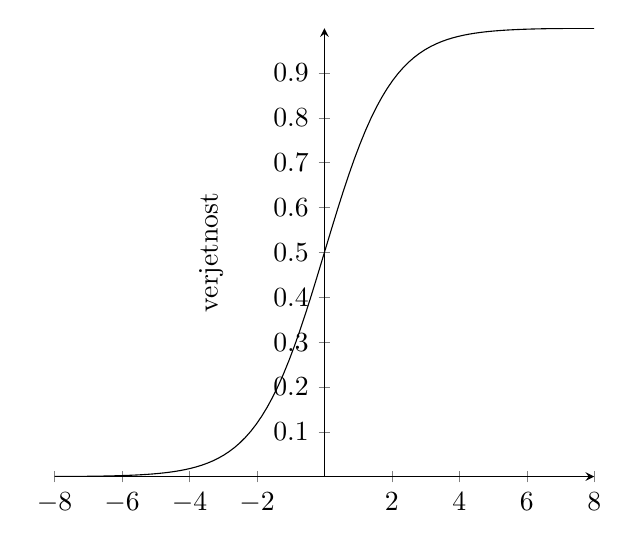
\begin{tikzpicture}
    \begin{axis}[
        axis lines = center,
        %xtick = {-10,-9,-8,...,9,10}
        ytick = {0,0.1,0.2,...,0.9,1},
        ylabel = verjetnost,
        y label style = {at={(axis description cs:0.25,.5)},rotate=90}%,anchor=south}
    ]
    \addplot [
        domain=-8:8, 
        samples=100, 
        color=black,
        ]
        {exp(x)/(1+exp(x))};
    %\addlegendentry{$x^2 + 2x + 1$}
    
    \end{axis}
\end{tikzpicture}
\caption{Graf sigmoide}
\label{fig:sigmoid}
\end{figure}
\end{center}

Če izpeljane izraze za verjetnost \refeq{p_i} upoštevamo v logaritemski funkciji verjetja, dobimo

\begin{align}
    \ell(\beta)  &= \sum_{i=1}^{n}\left( m_{i}\log{\frac{1}{1 + \exp{x_{i}^\top\beta}}}  + y_{i}\log{\left( \frac{\frac{\exp{x_{i}^{\top} \beta}}{1 + \exp{x_{i}^\top\beta}}}{\frac{1}{1 + \exp{x_{i}^\top\beta}}}  \right)} \right) \nonumber\\
                &= \sum_{i=1}^{n}\left( y_{i}(x_{i}^\top\beta) - m_{i}\log(1 + \exp{x_{i}^\top\beta})\right).
\end{align}
Od tod vidimo, da je naša funkcija verjetja odvisna le od parametrov $\beta$, vse ostalo nam je poznano. Da torej poiščemo maksimum in s tem
cenilko največjega verjetja, funkcijo odvajamo in zbirno funkcijo enačimo z 0
\[
    \frac{\partial}{\partial \beta}\ell(\beta) = \begin{bmatrix}
                                 \frac{\partial}{\partial \beta_{0}}L(\beta) \\
                                 \frac{\partial}{\partial \beta_{1}}L(\beta) \\
                                 \vdots \\
                                 \frac{\partial}{\partial \beta_{r}}L(\beta)
                        \end{bmatrix}.
\]
Pomembno je opaziti, da parametri $\beta$ vedno nastopajo ob pojasnjevalnih spremenljivkah linearno, zato bodo vse komponente enake oblike.
J-ta komponenta bo tako enaka
\begin{equation}
    \frac{\partial}{\partial \beta_{j}} \ell(\beta) = \sum_{i=1}^{n} \left(x_{ij}(y_{i} - m_{i}p_{i}(\beta))\right) = \sum_{i=1}^{n} \left(x_{ij}(y_{i} - \mu_{i})\right),~~j = 0,1,\ldots r,
\end{equation}
kjer smo upoštevali
\[
    \frac{\partial}{\partial \beta_{j}}(x_{i}^\top\beta) = \frac{\partial}{\partial \beta_{j}}\left(\beta_{0} + x_{i1}\beta_{1} + \ldots x_{ir}\beta_{r}\right) = x_{ij}
\]
ter
\begin{align}                                         
    \frac{\partial}{\partial \beta_{j}} \log(1 + \exp(x_{i}^\top\beta)) &= \frac{ \frac{\partial}{\partial \beta_{j}}\exp(x_{i}^\top\beta) }{1 + \exp(x_{i}^\top\beta)} \nonumber \\
    &= \frac{\exp(x_{i}^\top\beta)}{1 + \exp(x_{i}^\top\beta)} \frac{\partial}{\partial \beta_{j}} (x_{i}^\top\beta) \nonumber \\
    &=p_{i}(\beta)x_{ij}
\end{align}
in
\[
    m_{i}p_{i}(\beta) = \mu_{i}(\beta).
\]

Funkcijo zbira kot produkt matrik zapišemo
\begin{align}\label{prvi}
    \frac{\partial}{\partial \beta}\ell(\beta) = X^\top(y - \mu(\beta)).
\end{align}

Enačbe, ki jih s tem postopkom dobimo, v splošnem niso eksplicitno rešljive. Za reševanje se uporablja numerične metode, ki slonijo na Newtonovi iteraciji. Kot
bomo kasneje pokazali, je zanjo potrebno izračunati še drugi odvod, zato to storimo tu. Zopet odvajamo po komponentah, tako kot zgoraj. Najprej izračunajmo
\begin{align*}
    \frac{\partial p_{i}(\beta)}{\partial \beta_{k}} &= \frac{\partial}{\partial \beta_{k}} \frac{\exp{x_{i}^\top\beta}}{1+\exp{x_{i}^\top\beta}} \nonumber \\
        &= x_{ik}p_{i}(\beta)(1 - p_{i}(\beta)).
\end{align*}
Vse sedaj skupaj sestavimo v
\begin{align}
    \frac{\partial^2}{\partial \beta_{j}\partial\beta_{k}} \ell(\beta) &= - \sum_{i=1}^{n}\left(x_{ij}x_{ik}m_{i}p_{i}(\beta)(1-p_{i}(\beta))\right) \\
    &= -\sum_{i=1}^{n}\left(x_{ij}x_{ik}v_{i}(\beta)\right),~~j,k = 0,1,\ldots, r
\end{align}
kjer smo v drugi vrstici upoštevali  $\mathrm{Var}(Y_{i}) = v_{i}(\beta) = m_{i}p_{i}(1-p_{i}).$

Ostane nam le še dvojni odvod. Najprej si oglejmo
\[
    v(\beta) = \begin{bmatrix}
        v_{1}(\beta)  & & &\\
        & v_{2}(\beta) & & \\
        & & \ddots & \\
        & & & v_{n}(\beta)
    \end{bmatrix},
\]
iz tega potem takoj sledi, da je
\begin{equation} \label{drugi}
    \frac{\partial}{\partial \beta}\ell(\beta) = -X^\top v(\beta)X,
\end{equation}
torej element v $j$-ti vrstici in $k$-tem stolpcu je $\sum_{i=1}^{n}x_{ij}x_{ik}v_{i}(\beta).$

\subsection{Obstoj rešitve enačb verjetja v logističnem modelu}

V prejšnjem odseku smo izpeljali enačbe verjetja za logistično regresijo in pripomnili, da v splošnem niso analitično rešljive. Porodi pa se vprašanje,
kdaj rešitev pravzaprav sploh obstaja? Izkaže se, da je obstoj in enoličnost rešitve v logističnem modelu moč dokazati iz podatkov. Sledeči podrazdelek temelji na članku
\cite{albert1984existence}.

Zopet bomo vpeljali nekaj novih oznak. Imejmo $n$ neodvisnih opazovanj vektorja dimenzije $p$ in določimo $(x,H),$ kjer je $x^\top = (x_{0},\ldots,x_{r}),x_{0}\equiv 1,$
$H$ pa je spremenljivka, ki zavzame vrednosti $H_{1},\ldots,H_{g}$ in pokaže kateri skupini pripada določeno opazovanje. V našem primeru je $g=2$, $H_{1}$ ustreza Bernoullijevi
enki, $H_{2}$ pa Bernoullijevi ničli.


Potrebujemo način za razvrščanje vektorjev v skupine. Vektor $x$ pripada skupini $H_{1}$ natanko tedaj, ko velja
\[
    \langle x,\beta \rangle \geq 0
\]
in skupini $H_{2}$ natanko tedaj, ko velja
\[
    \langle x,\beta \rangle \leq 0.
\]

Označimo še $E_{1} = \{i~\vline~y_{i} = 1\}$ in $E_{1} = \{i~\vline~y_{i} = 0\},$ torej indekse vrstic, kjer je element vektorja $Y$ enak nič oziroma 1.

Logaritemsko funkcijo verjetja v splošnem zapišemo kot
\[
    \ell(X,\beta) = \sum_{j=1}^{g}\sum_{i\in E_{j}}\log\left(\frac{1}{\sum_{t=1}^{g} \exp(\beta_{t}-\beta_{j})^\top x_{i}}\right),
\]

v našem primeru pa se poenostavi na
\begin{equation*}
\ell(X,\beta) = \sum_{i\in E_{1}} \log\left(\frac{1}{1+\exp(-\langle x_{i},\beta \rangle)}\right) + \sum_{i\in E_{2}}\log\left(\frac{1}{\exp(\langle x_{i},\beta \rangle) + 1}\right).
\end{equation*}

V nadaljevanju bomo ločeno obravnavali možnosti, kako so lahko podatki razporejeni glede na to, kateri skupini pripadajo. Podrobneje si bomo pogledali in narisali
primere, ko sta skupini dve - tedaj imamo tri možnosti:
\begin{itemize}
    \item podatki so popolnoma ločeni - popolna separacija
    \item podatki so popolnoma ločeni, vendar nekateri ležijo ravno na meji - nepopolna separacija
    \item podatki se prekrivajo - prekrivanje
\end{itemize}
Na podlagi tega lahko določimo ali rešitev enačb verjetja obstaja in ali je enolična.

\subsubsection{Popolna separacija}
Popolna separacija v podatkih je prisotna, če 
\[
    \exists \beta: \forall i \in E_{1}: \langle x_{i},\beta \rangle > 0,~
    \forall i \in E_{2}: \langle x_{i},\beta \rangle < 0
\]
%Torej obstaja vektor $\beta,$ ki nam podatke popolnoma loči na skupine. 
%V primeru dveh skupin se pogoj prevede na $\beta^\top x_{i}>0, i\in E_{1}$ in $\beta^\top x_{i}<0, i\in E_{2}.$


\begin{izrek}
    Če je v podatkih prisotna popolna separacija, cenilka največjega verjetja $\hat{\beta}$ ne obstaja in velja
    \[
        \sup_{\beta} \ell(X,\beta) = 0.
    \]
\end{izrek}

\begin{proof}
    Če tak $\beta$ obstaja, potem je
    \[
    \log F(X,\beta) = \sum_{i\in E_{1}} \log\left(\frac{1}{1+\exp(-\underbrace{\langle x_{i},\beta \rangle}_{>0})}\right) + \sum_{i\in E_{2}}\log\left(\frac{1}{\exp(\underbrace{\langle x_{i},\beta \rangle}_{<0}) + 1}\right).
    \]
    V log-verjetje vstavljamo $\lambda \cdot \beta$ in ko pošljemo $\lambda$ proti neskončnosti, gre zgornji izraz proti 0.
\end{proof}

Grafično si popolno separacijo predstavljamo takole
\begin{center}
    \begin{figure}[h!]
    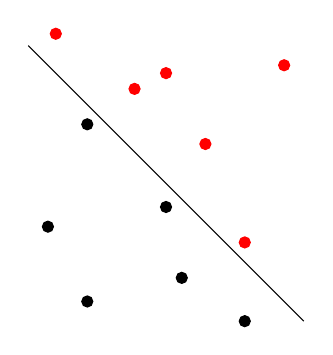
\begin{tikzpicture}
    %\draw (0,4) -- (0,0) -- (4,0);
    \draw (3.75,0.25) -- (0.25,3.75);
    \filldraw[black] (2.2,0.8) circle (2pt);
    \filldraw[black] (1,2.75) circle (2pt);
    \filldraw[black] (2,1.7) circle (2pt);
    \filldraw[black] (0.5,1.45) circle (2pt);
    \filldraw[black] (1,0.5) circle (2pt);
    \filldraw[black] (3,0.25) circle (2pt);
    
    \filldraw[red] (3,1.25) circle (2pt);
    \filldraw[red] (2,3.4) circle (2pt);
    \filldraw[red] (1.6,3.2) circle (2pt);
    \filldraw[red] (3.5,3.5) circle (2pt);
    \filldraw[red] (0.6,3.9) circle (2pt);
    \filldraw[red] (2.5,2.5) circle (2pt);
    
    \end{tikzpicture}
    \caption{Popolna separacija}
\end{figure}
\end{center}
kjer so s črno predstavljeni podatki v eni skupini, z rdečo pa v drugi.

\subsubsection{Nepopolna separacija}
Nepopolna separacija v podatkih je prisotna, če obstaja tak vektor $\beta$, da velja
\begin{equation}\label{nepopolnaSep}
    \forall i \in E_{1}: \langle x_{i},\beta \rangle \geq 0,~\forall i\in E_{2}: \langle x_{i},\beta \rangle \leq 0,
\end{equation}
pri čemer velja enakost za vsaj en $i$.

Kot je omenjeno že zgoraj, v tem primeru podatke lahko popolnoma ločimo, a nekateri ležijo popolnoma na meji. Lahko pa se zgodi, da je podatke možno ločiti na več načinov. V spodnjih
slikah sta obravnavana oba primera - ko imamo eno samo ločnico in ko jih je možno najti več.

Poglejmo si primer, ko je $g=2$. Označimo s $Q(\beta)$ tiste podatke, ki zadoščajo enakosti v \eqref{nepopolnaSep} in recimo, da je takih $r \neq 0$. Naj bo 
$X^{q}$ matrika teh opažanj dimenzij $r\times(p+1).$ Velja $X^{q}\beta=0,$ torej so vrstice v $X^{q}$ linearno odvisne in pripadajo podprostoru dimenzije $d \leq p$.
Velja tudi $d = rang(X^{q}).$ Če je $rang(X^{q}) = p,$ je torej ločnica med podatki enolična, kot na sliki \ref{fig:enolicna}, sicer pa je takih ločnic lahko več, kot vidimo v
sliki \ref{fig:neenolicna}.
\begin{center}
    \begin{figure}[h!]
    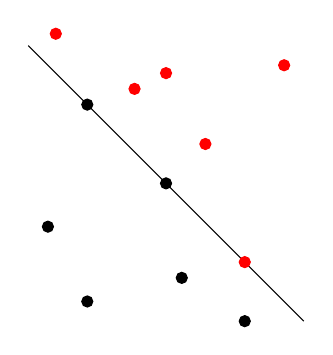
\begin{tikzpicture}
    %\draw (0,4) -- (0,0) -- (4,0);
    \draw (3.75,0.25) -- (0.25,3.75);
    \filldraw[black] (2.2,0.8) circle (2pt);
    \filldraw[black] (1,3) circle (2pt);
    \filldraw[black] (2,2) circle (2pt);
    \filldraw[black] (0.5,1.45) circle (2pt);
    \filldraw[black] (1,0.5) circle (2pt);
    \filldraw[black] (3,0.25) circle (2pt);
    
    \filldraw[red] (3,1) circle (2pt);
    \filldraw[red] (2,3.4) circle (2pt);
    \filldraw[red] (1.6,3.2) circle (2pt);
    \filldraw[red] (3.5,3.5) circle (2pt);
    \filldraw[red] (0.6,3.9) circle (2pt);
    \filldraw[red] (2.5,2.5) circle (2pt);
    
    \end{tikzpicture}
    \caption{Nepopolna separacija, prvi primer}
    \label{fig:enolicna}
\end{figure}
\end{center}

\begin{center}
    \begin{figure}%[h!]
    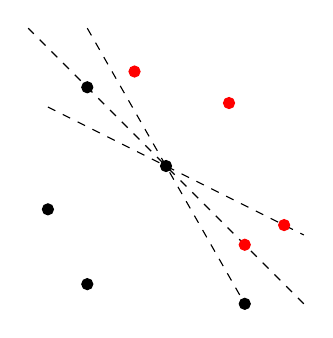
\begin{tikzpicture}
    %\draw (0,4) -- (0,0) -- (4,0);
    \draw[dashed] (3.75,0.25) -- (0.25,3.75);
    \draw[dashed] (1,3.75) -- (3,0.25);
    \draw[dashed] (0.5,2.75) -- (3.75,1.125);

    %\filldraw[black] (2.2,0.8) circle (2pt);
    \filldraw[black] (1,3) circle (2pt);
    \filldraw[black] (2,2) circle (2pt);
    \filldraw[black] (0.5,1.45) circle (2pt);
    \filldraw[black] (1,0.5) circle (2pt);
    \filldraw[black] (3,0.25) circle (2pt);
    
    \filldraw[red] (3,1) circle (2pt);
    \filldraw[red] (1.6,3.2) circle (2pt);
    \filldraw[red] (3.5,1.25) circle (2pt);
    \filldraw[red] (2.8,2.8) circle (2pt);
    
    \end{tikzpicture}
    \caption{Nepopolna separacija, drugi primer}
    \label{fig:neenolicna}
\end{figure}
\end{center}
\pagebreak
\subsubsection{Prekrivanje}
Če je v podatkih prisotno prekrivanje, torej ne padejo v nobeno od prejšnjih dveh kategorij, je sistem enačb verjetja rešljiv enolično.
\begin{center}
    \begin{figure}[h!]
    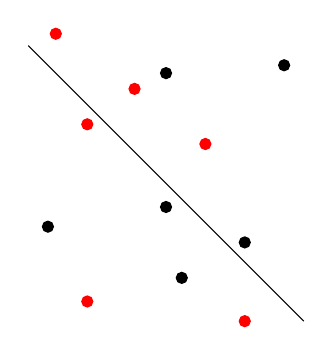
\begin{tikzpicture}
    %\draw (0,4) -- (0,0) -- (4,0);
    \draw (3.75,0.25) -- (0.25,3.75);
    \filldraw[black] (2.2,0.8) circle (2pt);
    \filldraw[red] (1,2.75) circle (2pt);
    \filldraw[black] (2,1.7) circle (2pt);
    \filldraw[black] (0.5,1.45) circle (2pt);
    \filldraw[red] (1,0.5) circle (2pt);
    \filldraw[red] (3,0.25) circle (2pt);
    
    \filldraw[black] (3,1.25) circle (2pt);
    \filldraw[black] (2,3.4) circle (2pt);
    \filldraw[red] (1.6,3.2) circle (2pt);
    \filldraw[black] (3.5,3.5) circle (2pt);
    \filldraw[red] (0.6,3.9) circle (2pt);
    \filldraw[red] (2.5,2.5) circle (2pt);
    
    \end{tikzpicture}
    \caption{Prekrivanje}
\end{figure}
\end{center}
Vidimo, da v tem primeru podatkov ni možno razdeliti na dve ločeni skupini

\subsection{Kanonični modeli v splošnem}
Kot bomo spoznali v sledečem razdelku, spada logistična regresija med tako imenovane modele s ">kanonično"< povezovalno funkcijo. 
Za vpeljavo tega ter nekaj ostalih pojmov pa potrebujemo nekaj dodatne teorije.

\subsubsection{Pomembnost kanoničnih povezovalnih funkcij}\label{kan}
Kot smo omenili že v uvodu, povezovalna funkcija opisuje relacijo med pričakovano vrednostjo opazovane spremenljivke in
sistematično komponento modela. Eksponentno družino in nekaj osnovnih zvez smo predstavili že v poglavju \ref{eksponentnaDruzina}.
%\[
%    f_{Y}(y; \theta, \phi) = \exp{\left(\frac{y\theta - b(\theta)}{a(\phi)} + c(y, \phi)\right)}.
%\]
%Enačbo logaritmiramo in dobimo
%\[
%    L(y;\theta) = \frac{y\theta-b(\theta)}{a(\phi)} + c(y;\phi),
%\]
%njen odvod, torej funkcija zbira pa je 
%\[
%    \frac{\partial}{\partial \theta} L(y;\theta) = \frac{y-b'(\theta)}{a(\phi)}.
%\]
Povezovalna funkcija posplošenega linearnega modela je kanonična, če je enaka naravnemu parametru eksponentne družine. V logistični regresiji je povezovalna funkcija logit,
v poglavju \ref{eksponentnaDruzina} pa smo pokazali, da je za binomsko porazdelitev to ravno naravni parameter. Logit je torej kanonična povezovalna funkcija v logističnem modelu.

V spodnji tabeli je navedenih še nekaj drugih primerov takih funkcij.

\begin{center}
    \begin{tabular}{ | c | c | c |}
        \hline
        Porazdelitev & $g(\mu)$ & Uporaba \\
        \hline
        Normalna & $id(\mu)$ &  Linearni odgovori\\
        Poissonova & $\log \mu$ & Število pojavitev \\
        Binomska & $\mathrm{logit}\mu$ & Binarni podatki\\
        Gamma & $-\frac{1}{\mu}$ & \\
        \hline
    \end{tabular}
\end{center}

%V sledečem razdelku bomo v namen poenostavljenja nekoliko spremenili notacijo. Logaritemsko funkcijo verjetja in njene odvode bomo sedaj upoštevali v smislu 
%le enega opazovanja, torej $y_{i} = y,$ za jasnost pa ohranili nekaj originalnih notacij - odvod po komponentah vektorja $\beta$ ter elemente matrike $\mathbf{X}$.
%
V sledečem razdelku smo zaradi poenostavljenja uporabili hibridne oznake. Logaritemsko funkcijo verjetja in njene odvode upoštevamo kot funkcijo le
enega opazovanja ($y_{i} = y$), odvode po komponentah $\beta$ pa še vedno pišemo z indeksi. Rezultate za celoten vzorec tako dobimo s seštevanjem po $i = 1,\ldots,n.$

Že v zgledu z logistično regresijo smo videli, da potrebujemo odvode logaritemske funkcije verjetja po parametrih $\beta.$ Uporabiti moramo verižno pravilo 
\[
    \frac{\partial \ell}{\partial\beta_{j}} = \left(\frac{\partial \ell}{\partial \theta}\right)\left(\frac{\partial \theta}{\partial\mu}\right)
    \left(\frac{\partial\mu}{\partial\eta}\right)\left(\frac{\partial\eta}{\partial\beta_{j}}\right).
\]
Lotimo se ga po korakih. Prvi faktor smo že v poglavju \ref{eksponentnaDruzina} izračunali kot $\frac{y-b'(\theta)}{a(\phi)}.$ Z uporabo $(b')^{-1}(\mu) = \theta$ in pravila za odvajanje inverzne funkcije 
dobimo $\frac{\partial \theta}{\partial\mu} = \frac{1}{b''(\theta)} = \frac{a(\phi)}{\mathrm{Var}(Y)},$ zadnji faktor pa bo kar vedno enak $x_{ij}.$ Tretji člen je odvisen
od povezovalne funkcije in se mu bomo posvetili nekoliko kasneje. Sestavimo vse skupaj in dobimo
\[
    \frac{\partial \ell}{\partial\beta_{j}} = \frac{y-\mu}{\mathrm{Var}(Y)}\frac{\partial \mu}{\partial\eta}x_{ij}.
\]

Opazimo: če imamo opravka s kanonično povezovalno funkcijo je $\eta = \theta.$ Torej namesto odvajanja po $\eta$ lahko $\mu$ odvajamo po $\theta$ in
dobimo $\frac{\partial\mu}{\partial\theta} = b''(\theta)$. Odvod se tako še dodatno poenostavi v
\begin{equation}
    \frac{\partial \ell}{\partial\beta_{j}} = \frac{y-\mu}{\mathrm{Var}(Y)}b''(\theta)x_{ij} = \frac{y-\mu}{a(\phi)}x_{ij}.
\end{equation}

Za numerične metode bomo potrebovali še druge odvode, kjer pa nam pomaga informacijska enakost iz dokaza trditve \ref{izp}.

Najprej izračunajmo pričakovano vrednost odvoda funkcije zbira
\begin{align*}
    -\mathbb{E}\left(\frac{\partial^2 \ell}{\partial\beta_{j}\partial\beta_{k}}\right) &= \mathbb{E}\left((\frac{\partial \ell}{\partial \beta_{j}})(\frac{\partial \ell}{\partial \beta_{k}})\right) \\
    &= \mathbb{E}\left(\left(\frac{y-\mu}{\mathrm{Var}(Y)}\right)^{2}\right)(\frac{\partial\mu}{\partial\eta})^{2}x_{ij}x_{ik} \\
    &= \frac{1}{\mathrm{Var}(Y)}(\frac{\partial\mu}{\partial\eta})^{2}x_{ij}x_{ik} \\
    &= \frac{b''(\theta)}{a(\phi)}x_{ij}x_{ik},
\end{align*}
kjer smo, tako kot v prejšnji enačbi, v prehodu v zadnjo vrstico upoštevali $\eta = \theta.$ 

Po drugi strani pa je običajen drugi odvod enak
\begin{align}\label{drugiOdvodZbira}
    \frac{\partial^2\ell}{\partial\beta_{j}\partial\beta_{k}} &= \frac{\partial}{\partial\beta_{k}}\{\left(\frac{\partial \ell}{\partial\theta}\right)\left(\frac{\partial \theta}{\partial\beta_{j}}\right)\} \nonumber \\
    &= \frac{\partial \ell}{\partial\theta}\left(\frac{\partial^2\theta}{\partial\beta_{j}\partial\beta_{k}}\right) + \left(\frac{\partial\theta}{\partial\beta_{j}}\right)\left(\frac{\partial^2\ell}{\partial\theta^2}\right)\left(\frac{\partial\theta}{\partial\beta_{k}}\right).
\end{align}
Lotimo se ga po korakih. Izračunali smo že, da je $\frac{\partial \ell}{\partial\theta} = \frac{y-b'(\theta)}{a(\phi)}.$ Drugi odvod je torej
\[
    \frac{\partial^2 \ell}{\partial\theta^2} = -\frac{b''(\theta)}{a(\phi)}.
\]
Za $\frac{\partial\theta}{\partial\beta_{j}}$ zopet v poštev pride verižno pravilo
\[
    \frac{\partial\theta}{\partial\beta_{j}} = \frac{\partial\theta}{\partial\mu}\frac{\partial\mu}{\partial\eta}\frac{\partial\eta}{\partial\beta_{j}} = \frac{1}{b''(\theta)}\frac{\partial\mu}{\partial\eta}x_{ij},
\]
v enaki obliki tudi za $\frac{\partial\theta}{\partial\beta_{k}},$ le da $x_{ij}$ zamenjamo z $x_{ik}.$
Drugi odvod funkcije zbira je z upoštevanjem zgornjega
\[
    \frac{\partial^2\ell}{\partial\beta_{j}\partial\beta_{k}} = \frac{y-b'(\theta)}{a(\phi)}\frac{\partial}{\partial\beta_{k}}\left(x_{ij}\frac{1}{b''(\theta)}\frac{\partial\mu}{\partial\eta}\right) + 
    \frac{1}{b''(\theta)^2}\left(\frac{\partial\mu}{\partial\eta}\right)^2\left(-\frac{b''(\theta)}{a(\phi)}\right)x_{ij}x_{ik}.
\]

Preostane računanje drugega faktorja prvega člena.
\begin{align*}
    \frac{\partial}{\partial\beta_{k}}\left(x_{ij}\frac{1}{b''(\theta)}\frac{\partial\mu}{\partial\eta}\right) &= x_{ij}\left(\frac{-b'''(\theta)}{b''(\theta)^2}\frac{\partial\mu}{\partial\eta}\frac{\partial\theta}{\partial\beta_{k}}
    +\frac{1}{b''(\theta)}\frac{\partial^2\mu}{\partial\eta^2}x_{ik}\right) \\
    &= x_{ij}\left(\frac{-b'''(\theta)}{b''(\theta)^2}\left(\frac{\partial\mu}{\partial\eta}\right)^2\frac{x_{ik}}{b''(\theta)} +
    \frac{1}{b''(\theta)}\frac{\partial^2\mu}{\partial\eta^2}x_{ik}\right).
\end{align*}
Splošna formula Hessejeve matrike je torej
\begin{multline}\label{splosniHesse}
    \frac{\partial^2\ell}{\partial\beta_{j}\partial\beta_{k}} = \frac{y-b'(\theta)}{a(\phi)} x_{ij}x_{ik}\left(\frac{-b'''(\theta)}{b''(\theta)^3}\left(\frac{\partial\mu}{\partial\eta}\right)^2 +
    \frac{1}{b''(\theta)}\frac{\partial^2\mu}{\partial\eta^2}\right) - \\
    -\frac{1}{b''(\theta)^2}\left(\frac{\partial\mu}{\partial\eta}\right)^2\frac{b''(\theta)}{a(\phi)}x_{ij}x_{ik}.
\end{multline}

Nadaljnje računanje bo odvisno od povezovalne funkcije. Če od tu naprej predpostavimo kanonično (in s tem $\theta = \eta$), se zgornji izraz nadaljuje v
\begin{multline*}
    \frac{x_{ij}x_{ik}}{b''(\theta)}\left(-b'''(\theta) + \frac{\partial}{\partial\eta}\left(\frac{\partial\mu}{\partial\eta}\right) \right) = \frac{x_{ij}x_{ik}}{b''(\theta)}\left(-b'''(\theta) + \frac{\partial}{\partial\eta}\left(\frac{\partial\mu}{\partial\theta}\right) \right) -\\
    -\frac{x_{ij}x_{ik}}{b''(\theta)}\left(-b'''(\theta) + \frac{\partial}{\partial\eta}\left(b''(\theta)\right) \right).
\end{multline*}

V drugem členu oklepaja upoštevamo kanonično povezovalno funkcijo
\[
    \frac{\partial}{\partial\eta}(b''(\theta)) = \frac{\partial}{\partial\theta}(b''(\theta)) = b'''(\theta).
\]
Sledi
\[
    \frac{x_{ij}x_{ik}}{b''(\theta)}\left(-b'''(\theta) + \frac{\partial}{\partial\eta}\left(b''(\theta)\right) \right) = \frac{x_{ij}x_{ik}}{b''(\theta)}\left(-b'''(\theta) + b'''(\theta) \right) = 0,
\]
torej za kanonične povezovalne funkcije prvi člen enačbe \refeq{drugiOdvodZbira} odpade in ostane le
\begin{align}
    \frac{\partial^2\ell}{\partial\beta_{j}\partial\beta_{k}} &= \frac{1}{b''(\theta)^2}\left(\frac{\partial\mu}{\partial\eta}\right)^2\left(-\frac{b''(\theta)}{a(\phi)}\right)x_{ij}x_{ik} \\
    &=-x_{ij}x_{ik}\frac{\partial^2\ell}{\partial\theta^2}.
\end{align}

Zaključimo
\begin{equation}\label{pv2odv}    
    \mathbb{E}\left(\frac{\partial^2\ell}{\partial\theta^2}\right) = \frac{\partial^2\ell}{\partial\theta^2}.
\end{equation}

Uporabnost zgornjega rezultata pa nam bo dalo poglavje o numeričnih metodah.

%\subsubsection{Poljubna povezovalna funkcija}
%Za poljubno povezovalno funkcijo smo v zgornjem razdelku pokazali
%\begin{align*}    
%    \frac{\partial}{\partial\beta_{j}}\ell &= \frac{y-\mu}{\mathrm{Var}(Y)}\left(\frac{\partial\mu}{\partial\eta}\right)x_{ij}\\
%    -\mathbb{E}\left(\frac{\partial^2L}{\partial\beta_{j}\partial\beta_{k}}\right) &= \frac{1}{\mathrm{Var}(Y)}\left(\frac{\partial\mu}{\partial\eta}\right)^2x_{ij}x_{ik}
%\end{align*}
%
\subsection{Probit regresija}
Probit regresija se uporablja v podobne namene kot logistična, torej za določanje verjetnosti in razvrščanje. Razvili so jo v tridesetih letih
dvajsetega stoletja, ime pa je skovanka -- pride iz angleških besed \textit{\textbf{prob}ability un\textbf{it}}. V glavnem se od logistične regresije
razlikuje v sistematičnem delu. Verjetnost pozitivnega izida torej po modelu predpostavljamo
\begin{equation}
    p_{i}(\beta) = \Phi (\beta_{0} + x_{i1}\beta_{1} + \ldots + x_{ir}\beta_{r}),
\end{equation}
kjer $\Phi$ predstavlja kumulativno porazdelitveno funkcijo standardne normalne slučajne spremenljivke. Ta seveda ni linearna,
podana je kot 
\[
    \Phi(x) = \frac{1}{\sqrt{2\pi}}\int_{-\infty}^{x}e^{\frac{-t^2}{2}}\,dt
\]
Očitno v tem primeru ne delamo s kanonično povezovalno funkcijo, kot smo to počeli v prejšnjem poglavju.

\subsubsection{Ocenjevanje parametrov probit regresije}\label{ocenpar_probit}
Podobno kot v logističnem modelu se bomo ocenjevanja parametrov lotili po metodi največjega verjetja.

Za sistematični del modela privzemimo binomsko porazdeljene slučajne spremenljivke s parametroma $\mathrm{Bin}(m_{i},p_{i}(\beta))$,
verjetnost pozitivnega izida pa izrazimo z
\[
    P(Y_{i} = y_{i}) = \binom{m_{i}}{y_{i}}p_{i}(\beta)^{y_{i}}(1 - p_{i}(\beta))^{m_{i} - y_{i}} = \binom{m_{i}}{y_{i}} (\Phi(x_{i}^\top \beta)^{y_{i}})(1 - \Phi(x_{i}^\top \beta))^{m_{i} - y_{i}} 
\]
Funkcijo verjetja tako kot zgoraj izrazimo z gostotami posameznih komponent
\[
    L(\beta) = \prod_{i=1}^{n} \binom{m_{i}}{y_{i}} \Phi(x_{i}^\top\beta)^{y_{i}}(1 - \Phi(x_{i}^\top\beta))^{m_{i} - y_{i}},
\]
kjer binomski simbol izpustimo zaradi enostavnejšega pisanja. Zgornjo enačbo logaritmiramo in dobimo
\begin{equation}
    \log(L(\beta)) = \ell(\beta) = \sum_{i = 1}^{n}\left(y_{i}\log\Phi(x_{i}^\top\beta) + (m_{i} - y_{i})\log(1 - \Phi(x_{i}^\top\beta)) \right)
\end{equation}

Izpeljava enačb verjetja v probit modelu je idejno zelo podobna tisti v razdelku \ref{ocenpar_logit}, direktno pa lahko uporabimo tudi zaključke prejšnjega razdelka. Funkcija zbira je

\[
    \frac{\partial \ell_{i}}{\partial\beta_{j}} = \frac{y_{i} - \mu_{i}}{\mathrm{Var}(Y)}\frac{\partial\mu_{i}}{\partial\eta_{i}}x_{ij} = \frac{y-m_{i}\Phi(x_{i}^\top\beta)}{\Phi(x_{i}^\top\beta)(1-\Phi(x_{i}^\top\beta))}\phi(x_{i}^\top\beta)x_{ij},
\]

rešujemo pa sistem

\begin{equation}
    \sum_{i = 1}^{n}\frac{\partial \ell_{i}}{\partial\beta_{j}} = 0,~~j=0,1,\ldots,r
\end{equation}
Te enačbe v splošnem niso rešljive analitično in zopet se bomo morali poslužiti numeričnih metod, za katere potrebujemo še druge odvode.

Po oznakah iz poglavja \ref{eksponentnaDruzina} je za binomsko porazdelitev s parametroma $n$ in $p$
\[
    b(\theta) = n\log(1+e^{\theta}),~\theta = \log\left(\frac{p}{1-p}\right).
\]

Potrebovali bomo prve tri odvode funkcije $b$
\begin{align*}
    b'(\theta) &= m_{i}\Phi(x_{i}^\top\beta) \\
    b''(\theta) &= m_{i}\Phi(x_{i}^\top\beta)1-\Phi(x_{i}^\top\beta) \\
    b'''(\theta) &= m_{i}\Phi(x_{i}^\top\beta)(1-\Phi(x_{i}^\top\beta))(1-2\Phi(x_{i}^\top\beta)),
\end{align*}
in pa odvode $\tfrac{\partial\mu}{\partial\eta}$
\begin{align*}
    \mu_{i} &= m_{i}\Phi(\eta) \\
    \frac{\partial\mu_{i}}{\partial\eta} &= m_{i}\phi(\eta) \\
    \frac{\partial^2\mu_{i}}{\partial\eta^2} & = -m_{i}\phi(\eta)\eta.
\end{align*}

Uporabimo prej izpeljano zvezo \refeq{splosniHesse} za Hessejevo matriko in dobimo
\begin{multline*}
    \frac{\partial^2}{\partial\beta_{j}\partial\beta_{k}}\ell(\beta) = \sum_{i = 1}^{n}
    x_{ij}\frac{(y_{i}-m_{i}p_{i})(-\phi(x_{i}^\top\beta)x_{i}^\top\beta) - m_{i}\phi(x_{i}^\top\beta)^2}{p_{i}(1-p_{i})}x_{ik} - \\
    -x_{ij}\frac{\phi(x_{i}^\top\beta)^2(1-2p_{i})}{(p_{i}(1-p_{i}))^2}x_{ik},
\end{multline*}
kjer upoštevamo $p_{i} = \Phi(x_{i}^\top\beta).$
%\frac{\partial^2}{\partial\beta_{j}\partial\beta_{k}}L(\beta) &= \sum_{i = 1}^{n}x_{ij}\left(-x_{i}^\top\beta x_{ik} \phi(x_{i}^\top\beta)\frac{y_{i}-m_{i}}{\Phi(x_{i}^\top\beta)(1-\Phi(x_{i}^\top\beta))}
%+\phi(x_{i}^\top\beta)^2x_{ik}\frac{2y_{i} - m_{i}\Phi(x_{i}^\top\beta)^2 - y_{i}}{(\Phi(1-\Phi(x_{i}^\top\beta)))^2}\right) \\
%&= \sum_{i=1}^{n}x_{ij}\frac{\phi(x_{i}^\top\beta)}{\Phi(x_{i}^\top\beta)(1-\Phi(x_{i}^\top\beta))}\left(\phi(x_{i}^\top\beta)\frac{2y_{i} - m_{i}\Phi(x_{i}^\top\beta)^2 - y_{i}}{(\Phi(1-\Phi(x_{i}^\top\beta)))}
%-(x_{i}^\top\beta)(y_{i}-m_{i}\Phi(x_{i}^\top\beta)) \right)x_{ik}

Zopet je koristno enačbe zapisati v matrični obliki. Za funkcijo zbira definirajmo vektor faktorjev
\[
    s = \begin{bmatrix}
        \phi(x_{1}^\top\beta)\frac{y_{1}-m_{1}\Phi(x_{1}^\top\beta)}{\Phi(x_{1}^\top\beta)(1-\Phi(x_{1}^\top\beta))} \\
        \vdots \\
        \phi(x_{n}^\top\beta)\frac{y_{n}-m_{n}\Phi(x_{n}^\top\beta)}{\Phi(x_{n}^\top\beta)(1-\Phi(x_{n}^\top\beta))} \\
    \end{bmatrix}
\]
in tako funkcijo zbira poenostavimo v
\[
    \frac{\partial}{\partial\beta}L(\beta) = X^\top s.
\]

Na podoben način se lotimo tudi Hessejeve matrike. Definiramo diagonalno matriko, kjer so na diagonali členi (zopet upoštevajoč zgornjo oznako $p_{i}$)
\[
    h_{i} = \frac{(y_{i}-m_{i}p_{i})(-\phi(x_{i}^\top\beta)x_{i}^\top\beta) - m_{i}\phi(x_{i}^\top\beta)^2}{p_{i}(1-p_{i})}
    -\frac{\phi(x_{i}^\top\beta)^2(1-2p_{i})}{(p_{i}(1-p_{i}))^2}
\]
torej $\mathbf{H} = diag(h_{1},\ldots,h_{n})$ in Hessejevo matriko zapišemo v preglednejši obliki
\[
    \frac{\partial^2}{\partial\beta^2} \ell(\beta) = X^\top \mathbf{H}X
\]
Končno, Newtonova metoda za iskanje ničel funkcije zbira z uporabo vseh zgornjih oznak
\begin{equation}
    \beta_{i+1} = \beta_{i} - (X^\top \mathbf{H} X)^{-1}X^\top s.
\end{equation}


\section{Numerične metode}
V sledečih razdelkih si bomo od bliže pogledali nekaj numeričnih metod, uporabljenih v kasnejših zgledih. Te metode slonijo na stoletja starih
idejah, ki smo jih spoznali tekom študija, uporabljajo pa se tudi v številnih praktičnih aplikacijah.
\subsection{Newton -- Raphsonova metoda} \label{nr}
Newton -- Raphsonova (oziroma le Newtonova) metoda je bila v osnovi razvita za iskanje ničel funkcije. Spada v razred \textit{navadnih iteracij}, torej metod za iterativno
reševanje enačb $f(x) = 0.$% ki jih prevedemo na $g(x) = x,$ izberemo začetni približek $x_{0}$ in ponavljamo 
%\[
%    x_{r+1} = g(x_{r}).
%\]

V najosnovnejši (ter najpogostejši) verziji za iskanje
ničle funkcije ene spremenljivke začnemo v neki točki, naslednjo pa izberemo v presečišču tangente, izračunane v 
tej točki, z x-osjo. Postopek tako iterativno nadaljujemo. Ideja je torej sila preprosta.
Predpostavimo odvedljivost funkcije na nekem intervalu in recimo, da imamo trenuten približek $x_{n}.$~Razvijmo sedaj funkcijo v Taylorjev
polinom prve stopnje okoli $x_{n}$:
\[
    f(x) \approx f(x_{n}) + f'(x_{n})(x - x_{n})
\]
Presečišče najdemo, če zgornjo enačbo enačimo z 0 in dobimo znano formulo
\[
    x_{n+1} = x_{n} - \frac{f(x_{n})}{f'(x_{n})}.
\]
Metoda konvergira za začetne približke dovolj blizu ničli in v neki okolici ničle konvergira s kvadratično hitrostjo. 
Na težave lahko naletimo v več primerih. Najprej, blizu stacionarne točke metoda odpove, saj bi delili z 0 (oziroma vrednostmi blizu ničle, kar je numerično nestabilno).
Problem lahko predstavljata tudi računanje odvoda ter dejstvo, da za slabe začetne približke ničle morda ne bomo našli. S temi 
težavami se bomo soočili v nadaljevanju.

\subsubsection{Newton--Raphsonova metoda v višjih dimenzijah}
Newtonovo metodo se da enostavno posplošiti za iskanje ničel vektorskih funkcij. Recimo, da imamo funkcijo $F:\mathbb{R}^{n} \rightarrow \mathbb{R}^{n}$ in iščemo tak
vektor $x^{*} \in \mathbb{R}^{n},$ za katerega bo \\ $F(x^{*}) = (f_{1}(x^{*}),\ldots,f_{n}(x^{*})) = (0,\ldots,0).$
Podobno kot zgoraj tvorimo zaporedje
\[
    x^{(r+1)} = x^{(r)} - JF(x^{(r)})^{-1}F(x^{(r)}),~r=0,1,\ldots
\]
kjer smo z \textit{JF} označili Jacobijevo matriko. V praksi njenega inverza ne računamo, temveč uvedemo premike in rešujemo sistem enačb
\begin{align*}
    JF(x^{(r)}) h &= -F(x^{(r)}),\\
    x^{(r+1)} &= x^{(r)} + h,~r=0,1,\ldots
\end{align*}
od koder izračunamo vektor premikov $h \in \mathbb{R^n}$ in nato posodobimo prejšnji približek.

Izpeljava je podobna tisti v eni dimenziji, preko razvoja v Taylorjevo vrsto. Recimo, da so vse komponente funkcije $F$ dvakrat zvezno odvedljive v okolici rešitve. Potem razvijemo
\[
    f_{i}(x+h) = f_{i}(x) + \sum_{k=1}^{n} \frac{\partial f_{i}(x)}{\partial x_{k}}h_{k} + \ldots,~i=1,\ldots,n
\]
Želimo, da bo $f_{i}(x+h) = 0$ za vsak $i$, zanemarimo člene od kvadratnega dalje in rešujemo sistem za premike
\[
    \begin{bmatrix}
        \frac{\partial f_{1}(x)}{\partial x_{1}} & \cdots & \frac{\partial f_{1}(x)}{\partial x_{n}} \\
        \vdots & & \vdots \\
        \frac{\partial f_{n}(x)}{\partial x_{1}} & \cdots & \frac{\partial f_{n}(x)}{\partial x_{n}}
    \end{bmatrix}
    \begin{bmatrix}
        h_{1} \\
        \vdots\\
        h_{n}
    \end{bmatrix} 
    = -
    \begin{bmatrix}
       f_{1}(x) \\
       \vdots \\
       f_{n}(x)
    \end{bmatrix}.
\]
V okolici rešitve enačbe ima metoda kvadratično konvergenco, težava pa je v iskanju začetnega približka.

Imamo torej algoritem za iskanje ničel, v luči iskanja cenilke največjega verjetja pa bi želeli algoritem, ki poišče ekstrem funkcije.
%Recimo, da imamo logaritemsko funkcijo verjetja $\ell$, in trenutni približek $\theta_{n}$. Razvijmo funkcijo okoli približka v Taylorjev polinom
%druge stopnje:
%\begin{align}\label{taylor}
%    \ell(\theta) \approx \ell(\theta_{n}) + \frac{\partial}{\partial\theta}\ell(\theta_{n})(\theta - \theta_{n}) + \frac{1}{2}(\theta - \theta_{n})^\top \frac{\partial^2}{\partial\theta^2}\ell(\theta_{n})(\theta - \theta_{n}) 
%\end{align}
V našem primeru iščemo maksimum logaritemske funkcije verjetja $\ell.$ Tega se lotimo tako, da njen gradient enačimo z nič
\[
    \frac{\partial}{\partial\theta} \ell(\theta_{n}) + \frac{\partial^2}{\partial\theta^2}\ell(\theta_{n})(\theta - \theta_{n}) = 0
\]
in izrazimo naslednji približek
\[
    \theta_{n + 1} = \theta_{n} - \left(\frac{\partial^2}{\partial\theta^2}\ell(\theta_{n})\right)^{-1}\frac{\partial}{\partial\theta}\ell(\theta_{n}).
\]
%Te enačbe so direktna uporaba Newtonove metode za višje dimenzije, ki jo bomo podrobneje razložili nekoliko kasneje.
S tem postopkom imamo lahko dva problema. Prvič, drugi odvod (Hessian) funkcije je lahko zahtevno računati in invertirati, za kakšen $\theta_{n}$ morda sploh ne obstaja.
Drugič, Newtonova metoda ni naraščajoč algoritem in ne velja nujno $\ell(\theta_{n}) < \ell(\theta_{n+1}).$ Mi pa bi želeli algoritem, ki bo konvergiral globalno (in ne le na nekem intervalu okoli rešitve).

Težavo z računanjem inverza rešimo tako, da namesto invertiranja problem prevedemo na reševanje sistema enačb za premik:
\begin{align}\label{newtoneq}
    x_{n + 1} &= x_{n} + p_{n} \nonumber\\
    \frac{\partial^2}{\partial\theta^2}\ell(\theta_{n})p_{n} &= -\frac{\partial}{\partial\theta} \ell(\theta_{n})
\end{align}
Zadnji vrstici v \eqref{newtoneq} rečemo tudi \textit{Newtonova enačba}.
Radi bi še dosegli, da bi se Newtonov algoritem premikal v eno smer, torej naraščal ali padal. S tem bi vedeli, kaj se bo zgodilo v iteraciji in lažje predvideli morebitne
nevšečnosti. Newtonova metoda za iskanje minimuma (maksimuma) funkcije je optimizacijski problem drugega reda in realna funkcija ima globalni minimum (maksimum) tam, kjer je
njen drugi odvod pozitiven, oziroma v primeru funkcij več spremenljivk, kjer je njen Hessian pozitivno definiten (in je tam gradient enak nič). Če bi torej imeli
strogo pozitivno definitno matriko, bi bil ta optimizacijski problem konveksen in kot tak rešljiv globalno (veljati morajo še pogoji Karush-Kuhn-Tuckerja, vendar je to skoraj vedno res).
Imejmo torej v točki $x^{*}$ pozitivno definitno Hessejevo matriko $H.$~Zapišimo Taylorjev polinom druge stopnje okoli te točke
\[
    f(x^{*} + s) = f(x^{*}) + \frac{\partial}{\partial\theta} f(x^{*})s + \frac{1}{2}s^\top \frac{\partial^2}{\partial\theta^2}f(x^{*})s.
\]
Če velja še pogoj prvega reda, torej $\frac{\partial}{\partial\theta} f(x^{*}) = 0,$~imamo
\[
    f(x^{*} + s) = f(x^{*}) + \frac{1}{2}s^\top \frac{\partial^2}{\partial\theta}f(x^{*})s,
\]
kar pomeni, da se vrednost funkcije vedno poveča, če se premaknemo iz stacionarne točke $x^{*}$~(drugi člen je vedno pozitiven zaradi pozitivne definitnosti).
Tako vidimo, da imamo strogo padajoč algoritem.

\subsubsection{Potencialne težave Newtonove metode}
Newtonova metoda ima mnogo pozitivnih plati, vendar pa je iz določenih vidikov precej občutljiva. Morda najbolj očiten problem je slaba izbira začetne točke iteracije. Če je ta
stacionarna točka obravnavane funkcije, nam metoda narekuje deljenje z 0, kar pa seveda nima smisla. Očiten primer bi bil iskanje ničle funkcije $f(x) = 1+x^2$ z začetnim približkom $x_{0} = 0.$
Na pamet takoj vidimo, da so ničle v $1$ in $-1$, če pa bi upoštevali iteracijo, bi dobili
\[
    x_{1} = x_{0} - \frac{f(x_{0})}{f'(x_{0})} = 0 - \frac{1}{0}.   
\]
Enaka težava seveda nastopi, če v sledečih korakih dobimo stacionarno točko oziroma se ji približujemo in tako delimo z vedno manjšimi števili, kar pa vodi v vselej slabše približke.

Sicer redkeje se lahko zgodi tudi, da se približki ">zaciklajo"<. Primer take funkcije je $f(x) = x^3 - 2x + 2,$ če za začetni približek vzamemo 0. Tako v zaporednih korakih najprej dobimo
$x_{1} = 1$ in nato $x_{2} = 0$, kar pa je seveda naša začetna točka. Obstajajo okolice teh dveh točk, ki vedno konvergirajo v ta dvojni cikel in ne k iskani ničli. V splošnem 
zna biti obnašanje takega zaporedja precej zapleteno, imenuje se Newtonov fraktal in vanj se tu ne bomo spuščali.

Naslednja težava lahko nastopi, če se odvod naše funkcije lokalno ne obnaša dovolj ">lepo."< Prvič, odvod v ničli morda ne obstaja. Enostaven primer tega je 
$f(x) = \sqrt[3]{x}.$ Izračunamo
\[
    x_{n+1} = x_{n} - \frac{x_{n} ^ {\nicefrac{1}{3}}}{\frac{1}{3}x_{n}^{1 - \nicefrac{1}{3}}} = -2x_{n},
\]
in vidimo, da za vsak začetni približek različen od nič metoda divergira. Splošneje, podoben rezultat dobimo za vsako funkcijo oblike $f(x) = \lvert x \rvert^{\alpha}, 0 < \alpha < \frac{1}{2},$
za $\alpha = \frac{1}{2}$ pa metoda sicer ne divergira, vendar se kot v prejšnjem primeru zacikla in ne pridemo do rešitve.

V zgoraj naštetih primerih torej Newtonova metoda ne konvergira k iskani ničli. Smiselno sledi vprašanje, katerim pogojem mora biti zadoščeno, da 
vendarle dobimo pravilno rešitev. To nam poda sledeči izrek, ki zagotavlja konvergenco, če je iteracijska funkcija v okolici negibne točke skrčitev.
\begin{izrek} 
    Naj za iteracijsko funkcijo velja $g(\alpha) = \alpha$ in naj na intervalu $I = [ \alpha - \delta,\alpha + \delta ]$ zadošča Lipschitzovemu pogoju
    \[
        \lvert g(x) - g(y) \rvert \leq m \lvert x - y \rvert
    \]
    za konstanto 0 $\leq m < 1$ in poljubna $x,y \in I.$ Potem za vsak začetni približek $x_{0} \in I$ zaporedje $x_{r+1} = g(x_{r}), r \geq 1$ konvergira k $\alpha$. Poleg tega veljata
    tudi oceni
    \begin{equation}\label{prva_neenakost}
        \lvert x_{r} - \alpha \rvert \leq m^{r}\lvert x_{0} - \alpha \rvert
    \end{equation}
    in
    \begin{equation}
        \lvert x_{r+1} - \alpha \rvert \leq \frac{m}{1-m} \lvert x_{r} - x_{r-1} \rvert
    \end{equation}
\end{izrek}
\begin{proof}
    Označimo z $\varepsilon_{r} = x_{r} - \alpha $ napako približka $x_{r}.$ Velja
    \[
        \lvert \varepsilon_{r} \rvert = \lvert x_{r} - \alpha \rvert = \lvert g(x_{r-1}) - g(\alpha) \rvert \leq m\lvert x_{r-1} - \alpha \rvert = m \varepsilon_{r-1}.
    \]
    Ta postopek nadaljujemo in sledi
    \[
        \lvert \varepsilon_{r} \rvert \leq m \lvert \varepsilon_{r-1} \rvert \leq m^{2} \lvert \varepsilon_{r-2} \rvert \leq \ldots \leq m^{r} \lvert\varepsilon_{0} \rvert,
    \]
    koder vidimo oceno \eqref{prva_neenakost}.

    Za drugo neenakost pa si oglejmo
    \[
        \lvert x_{r+1} - \alpha \rvert \leq \lvert x_{r+1} - x_{r+2} \rvert + \lvert x_{r+2} - x_{r+3} \rvert + \ldots
    \]
    Upoštevamo še
    \[
        \lvert x_{r+k} - x_{r+k+1} \rvert = \lvert g(x_{r+k-1}) - g(x_{r+k}) \rvert \leq m \lvert x_{r+k-1} - x_{r+k} \rvert \leq \ldots \leq m^{k}v\lvert x_{r-1} - x_{r}\rvert 
    \]
    in končno dobimo
    \[
        \lvert x_{r+1} - \alpha\rvert \leq (m + m^2 + \cdots)\lvert x_{r-1} - x_{r}\rvert = \frac{m}{1-m}\lvert x_{r-1} - x_{r}\rvert
    \]
\end{proof}

Dodatno informacijo o območju konvergence navadne iteracije nam dajo tudi vrednosti odvoda iteracijske funkcije, o čemer govori naslednji izrek.
\begin{izrek}
    Naj bo iteracijska funkcija zvezno odvedljiva v negibni točki $\alpha$ in naj velja $\lvert g'(\alpha) \rvert < 1.$ Potem obstaja okolica I negibne točke,
    da za vsak začetni približek $x_{0} \in I$ iteracija konvergira k $\alpha.$
\end{izrek}
\begin{proof}
    Odvod je po predpostavki na neki okolici $\alpha$ strogo manjši od 1 in zaradi zveznosti obstajata $\delta > 0$ in konstanta $m < 1,$ da je $\lvert g'(x) \rvert < m < 1$ za $x \in I,$
    kjer z $I$ označimo $[\alpha - \delta,\alpha + \delta ].$ Potem po Lagrangeovem izreku velja $\lvert g(x) - g(y) \rvert \leq \lvert g'(\xi) \rvert \dot \lvert x - y \rvert,$
    za poljubna $x,y \in I.$ Ker je odvod na tem intervalu manjši od 1 sledi, da je funkcija g Lipschitzova in zato po \eqref{prva_neenakost} iteracija konvergira.
\end{proof}

\subsubsection{Asimptotsko obnašanje in konvergenca}
Kot je pri numeričnih metodah to običajno, nas zanima njihovo obnašanje po več ponovitvah iteracije. Pomembno je, kako hitro pridemo do rešitve, saj želimo računanje čim manjkrat
ponoviti in dobiti najboljši možen rezultat.

Definirajmo \textit{red konvergence}. Idejno je to število točnih decimalnih mest, ki jih pridobimo z vsakim korakom iteracije. 
\begin{definicija}\label{red_konv}
    Naj zaporedje $(x_{r})$ konvergira k $\alpha.$ Red konvergence je enak p, če obstajata taki števili $C_{1}, C_{2},$ da velja
    \[
        C_{1}\lvert x_{r} - \alpha \rvert ^{p} \leq \lvert x_{r+1} - \alpha \rvert \leq C_{2} \lvert x_{r} - \alpha \rvert^{p}.
    \]
    Ekvivalentno: red konvergence je p, če obstaja tako število $C > 0,$ da
    \[
        \lim_{r\to\infty} \frac{\lvert x_{r+1} - \alpha\rvert}{\lvert x_{r} - \alpha\rvert^{p}} = C.
    \]
\end{definicija}

Red konvergence navadne iteracije je običajno precej enostavno določiti. Metodo nam daje izrek
\begin{izrek}
    Naj bo iteracijska funkcija g v okolici svoje fiksne točke p-krat zvezno odvedljiva in $\lvert g'(\alpha) \rvert \leq 1, g^{(k)}(\alpha) = 0\text{ za }k = 1,\ldots,p-1 \text{ in }
    g^{(p)}(\alpha) \neq 0.$ Potem ima iterativna metoda lokalno red konvergence p.
\end{izrek}
\begin{proof}
    Razvijmo $g$ v Taylorjevo vrsto okrog $\alpha$
    \[
        x_{r+1} = g(x_{r}) = \alpha + \frac{1}{p!}(x_{r} - \alpha)^{p}g^{(p)}(\xi),
    \]
    kjer $\xi$ leži med $x_{r}$ in $\alpha.$ Ocenimo odvod navzgor in navzdol ter s tem dobimo konstanti $C_{1},C_{2}$ iz \ref{red_konv}.
\end{proof}

Pa poskusimo sedaj določiti red konvergence Newtonove metode. Označimo
\[
    g(x) = x - \frac{f(x)}{f'(x)}.
\]
Odvajamo in dobimo
\[
    g'(x) = \frac{f(x)f''(x)}{(f'(x))^{2}}.
\]
Vidimo, da je potrebno ločiti dva primera:
\begin{itemize}
    \item Če je $\alpha$ enostavna ničla funkcije $f,$ je $g'(\alpha)=0$ in je konvergenca vsaj kvadratična. Z nadaljnjim računom dobimo
    \[
        g''(\alpha) = \frac{f''(\alpha)}{f'(\alpha)},
    \]
    in vidimo, da je pri $f''(\alpha) \neq 0$ konvergenca kvadratična. Sicer postopek nadaljujemo, dokler ne najdemo prvega odvoda z vrednostjo v $\alpha$ 0.
    \item Če je $\alpha$ m-kratna ničla pa velja
    \[
        \lim_{x\to\alpha} g'(x) = 1 - \frac{1}{m},
    \]
    od koder sledi linearna konvergenca. Dokažimo drugo alinejo.
    \begin{proof}
        Ker je $\alpha$ m-kratna ničla, je prvih $m-1$ odvodov funkcije $f$ enakih 0. Opazimo, da moramo $(2m-2)$-krat uporabiti l'Hospitalovo pravilo, da dobimo neničeln ulomek
        \begin{equation*}
            \lim_{x\to\alpha} g'(x) = \lim_{x\to\alpha} \frac{f(x)f''(x)}{(f'(x))^{2}}
            = \lim_{x\to\alpha} \frac{\sum_{k=0}^{2m-2}\binom{2m-2}{k}f^{(k)}(x)f^{(2m-2)-k+2}(x)}{\sum_{k=0}^{2m-2}\binom{2m-2}{k}f^{(2m-2-k+1)}(x)f^{(k+1)}(x)},
        \end{equation*}
        v imenovalcu ostane le $m$-ti člen, v števcu pa $(m-1)$-ti. Izračunamo
        \[
            \frac{\binom{2m-2}{m}(f^{(m)}(x))^{2}}{\binom{2m-2}{m-1}(f^{(m)}(x))^{2}} = \frac{\frac{(2m-2)!}{(m-2)!m!}}{\frac{(2m-2)!}{(m-1)!(m-1)!}} = \frac{(m-1)!(m-1)!}{(m-2)!m!} = \frac{m-1}{m},
        \]
        kar je ravno želeni rezultat.
    \end{proof}

\end{itemize}
\subsection{Fisherjeva zbirna metoda}
Fisherjeva zbirna metoda je variacija v prejšnjem razdelku opisanega Newton -- Raphsonovega algoritma, ki se v statistiki uporablja za numerično reševanje enačb 
verjetja. Poimenovana je po Ronaldu Fisherju, enemu najpomembenjših angleških statistikov dvajsetega stoletja.

Ponovimo najprej nekaj terminologije. Funkcija zbira je gradient logaritemske funkcije verjetja po ocenjevanem parametru.
Informacijska (oziroma Fisherjeva informacijska) matrika (angl. \textit{(Fisher) information matrix}) je definirana kot 
\[
    \mathrm{FI}(\theta) = \mathbb{E}\left(\left(\frac{\partial}{\partial\theta} \ell(\theta)\right) \left(\frac{\partial}{\partial\theta} \ell(\theta)\right)^\top \right) %= \mathrm{E}[\dot{\ell}(\theta) \dot{\ell}(\theta)^\top].
\]
Fisherjeva zbirna metoda je po zgornjih oznakah 
\begin{align}
    \theta_{n + 1} = \theta_{n} - \mathrm{FI}(\theta)^{-1}\left(\frac{\partial}{\partial\theta} \ell(\theta)\right)
\end{align}
%\subsubsection{Fisherjeva informacijska matrika in informacijska enakost}
%V sledečem razdelku bomo utemeljili uporabo Fisher scoring algoritma in prikazali njegovo glavno prednost pred običajno Newtonovo iteracijo, opisano v poglavju \ref{nr}.
%
%Ob določenih predpostavkah o gladkosti logaritemske funkcije verjetja (ki za eksponentno družino vedno držijo), bomo sedaj pokazali, da je pričakovana vrednost
%zbirne funkcije enaka nič. Funkcijo verjetja tu pišemo kot logaritem gostote slučajnega vektorja.
%\begin{align} \label{Ezbirne}
%    \mathrm{E}[\nabla L (\theta)] &= \int f_{\theta}(x) \nabla_{\theta}\log(f_{\theta}(x)) \,dx = \int f_{\theta}(x) \frac{\nabla f_{\theta}(x)}{f_{\theta}(x)} \,dx \nonumber \\
%        &= \int \nabla f_{\theta}(x) \,dx \overset{*}{=} \nabla \int f_{\theta}(x) \,dx = \nabla 1 = 0, 
%\end{align}
%kjer smo v enakosti $(*)$ zamenjali integracijo in odvajanje, kar po teoriji mere smemo - gostota porazdelitev eksponentne družine je zvezno odvedljiva. 
%Velja tudi
%\[
%    \nabla^{2} \log{f_{\theta}(x)} = \frac{\nabla^2 f_{\theta}(x)}{f_{\theta}(x)} - \frac{\nabla f_{\theta}(x) \nabla f_{\theta}(x)^\top }{f_{\theta}(x)^{2}} = 
%    \frac{\nabla^2 f_{\theta}(x)}{f_{\theta}(x)} - \dot{\ell}(\theta)\dot{\ell}(\theta)^\top,
%\]
%kjer smo v zadnji enakosti upoštevali
%\[
%    \nabla L (\theta) = \nabla \log(f_{\theta}(x)) = \frac{\nabla f_{\theta}(x)}{f_{\theta}(x)} 
%\]
%Povzemimo vse, kar smo dokazali v prejšnjih enačbah in imamo
%\begin{align}\label{infoeq}
%    I(\theta) &= \mathrm{E}[\nabla L(\theta)(\nabla L(\theta))^\top] =  -\int f_{\theta}(x) \nabla^2 \log f_{\theta}(x) \,dx+ \int \nabla^2 f_{\theta}(x) \,dx \nonumber \\
%    &= -\mathrm{E}[\nabla^2 \log f_{\theta}(x)] + \nabla^2\int \log f_{\theta}(x) \,dx = -\mathrm{E}[\nabla^2 \log f_{\theta}(x)]
%\end{align}
%Enačbi \eqref{infoeq} rečemo tudi \textit{informacijska enakost}. To nam bo koristilo pri dokazovanju enakosti med Newton -- Raphson algoritmom in Fisher scoringom za logistični model.
%Kot smo videli v prejšnjih poglavjih, želimo imeti pozitivno semi-definitno matriko in s tem monoton algoritem. Izkaže se, da je informacijska matrika ravno variančno-kovariančna matrika
%zbirne funkcije. Po enačbi \eqref{Ezbirne} se spomnimo, da je pričakovana vrednost zbirne funckije enaka 0. Potem takoj sledi
%\begin{align}
%    I(\theta) &= \mathrm{E}[\nabla L(\theta)\nabla L(\theta)^\top] \nonumber\\
%    &= \mathrm{E}[\left(\nabla L(\theta) - \mathrm{E}[\nabla L(\theta)]\right)\left(\nabla L(\theta) - \mathrm{E}[\nabla L(\theta)]\right)^\top] \nonumber \\
%    &= \mathrm{Var}[\nabla L(\theta)].
%\end{align}
%Variančno-kovariančne matrike pa so pozitivno semi-definitne.

\subsubsection{Ujemanje Newton-Raphsonovega algoritma in Fisherjeve zbirne metode za kanonične povezovalne funkcije}
Spomnimo se zaključkov poglavja \ref{kan}. Tam smo dokazali, da za modele s kanonično povezovalno funkcijo velja $\mathbb{E}(\frac{\partial^2\ell}{\partial\theta^2}) = \frac{\partial^2}{\partial\theta^2}\ell,$
po informacijski enakosti pa velja 
\begin{equation*}
    \mathrm{FI}(\theta) = \mathbb{E}\left((\frac{\partial}{\partial\theta} \ell)(\frac{\partial}{\partial\theta} \ell)^\top\right) = \mathbb{E}\left(\frac{\partial^2}{\partial\theta^2}\ell\right) = \frac{\partial^2}{\partial\theta^2}\ell \\
    \rightarrow \mathrm{FI}(\theta) = \frac{\partial^2}{\partial\theta^2}\ell,
\end{equation*}
torej je Fisherjeva informacija za kanonične modele enaka Hessejevi matriki logaritemske funkcije verjetja! Poleg tega velja še
\begin{align}
    \mathrm{FI}(\theta) &= \mathbb{E}[(\frac{\partial}{\partial\theta} \ell(\theta))(\frac{\partial}{\partial\theta} \ell(\theta))^\top] \nonumber\\
    &= \mathbb{E}[\left(\frac{\partial}{\partial\theta} \ell(\theta) - \mathbb{E}[\frac{\partial}{\partial\theta} \ell(\theta)]\right)\left(\frac{\partial}{\partial\theta} \ell(\theta) - \mathbb{E}[\frac{\partial}{\partial\theta} \ell(\theta)]\right)^\top] \nonumber \\
    &= \mathrm{Var}[\frac{\partial}{\partial\theta} \ell(\theta)],
\end{align}
variančno kovariančne matrike pa so pozitivno semidefinitne, kar pomeni da imamo konstanten algoritem.


Povzemimo; za kanonične povezovalne funkcije smo dokazali enakost med Fisherjevo informacijo in Hessejevo matriko. S tem se v enem koraku izognemo računanju matrike drugih 
odvodov in pridobimo pozitivno semidefinitno matriko v imenovalcu. Koristi uporabe kanoničnih povezovalnih funkcij so torej očitne.

\subsubsection{Fisherjeva zbirna metoda  v logističnem modelu}
Poglejmo za trenutek nazaj v razdelek \ref{ocenpar_logit}, natančneje k enačbam \eqref{prvi} in \eqref{drugi}. Iz prejšnjih razdelkov vemo tudi, da velja
\[
    \mathrm{FI}(\theta) = \mathbb{E}[-\frac{\partial^2}{\partial\theta^2} \ell(\theta)] \overset{\eqref{drugi}}{=} X^\top v(\theta)X = -\frac{\partial^2}{\partial\theta^2} \ell(\theta),
\]
kjer smo seveda uporabili že dokazano informacijsko enakost. Tako vidimo, da Fisherjeva zbirna metoda in Newton--Raphsonova metoda v primeru logistične regresije
res sovpadata, saj je matrika drugih odvodov ravno enaka informacijski matriki. Vse skupaj zapišemo kot
\begin{align}
    \hat{\theta}_{i+1} &= \hat{\theta}_{i} - (\frac{\partial^2}{\partial\theta^2} \ell(\hat{\theta}_{i}))^{-1} \frac{\partial}{\partial\theta} \ell(\hat{\theta}_{i}) \nonumber \\
    &= \hat{\theta}_{i} + (X^\top v(\hat{\theta}_{i}) X)^{-1}X^\top(y - \mu(\hat{\theta}_{i})).
\end{align}

\section{Primeri}
\subsection{Ocenjevanje parametrov v logističnem modelu}

V praktično usmerjenem delu naloge smo v Pythonu implementirali zgoraj opisani postopek Fisherjeve zbirne metode za binomsko porazdeljene slučajne
spremenljivke. Za delo smo uporabili knjižnici \texttt{NumPy} za računanje z matrikami in vektorji, reševanje sistemov enačb ter invertiranje in
knjižnico \texttt{pandas} za uvoz podatkov in njihovo začetno urejanje. Na koncu smo si s paketom \texttt{Pyplot} iz knjižnice \texttt{Matplotlib} rezultate izrisali.
V implementaciji smo popolnoma sledili izpeljanim enačbam v razdelkih \ref{ocenpar_logit} in \ref{ocenpar_probit}, zato jih tu ne bomo ponovno navajali.

\subsubsection{Algoritem za logistični model in rezultati}
Povežimo vso izpeljano teorijo v algoritem za ocenjevanje parametrov modela oblike
\[
    \mathrm{logit}(p) = X\beta,
\]
torej kanoničnega logističnega modela.
\begin{algorithm}[H]
    \caption{\textbf{function} LogitModel(iteracije, X, Y, $\beta_{zacetni}$, $\epsilon$)}
\begin{algorithmic}
    
    %\COMMENT 
    \STATE $p = \frac{\exp{(X^\top \beta_{zacetni})}}{1 + \exp{(X^\top \beta_{zacetni})}}$
    \STATE $V = p(1 - p)$ 
    \STATE $Score = X^\top (Y - p)$ 
    \STATE $Info = X^\top V X$ 
    
    \STATE \text{\textit{Reši sistem na h:}} $Info * h = Score$
    \STATE $\beta_{star} = \beta_{zacetni}$
    \STATE $\beta_{nov} = \beta_{star} + h$
    \WHILE{$i \leq \text{iteracije}$}
        
        \IF{$\beta_{nov} - \beta_{star} \geq \epsilon$}
            \STATE $p = \frac{\exp{(X^\top \beta_{nov})}}{1 + \exp{(X^\top \beta_{nov})}}$ 
            \STATE $V = p(1 - p)$ 
            \STATE $Score = X^\top (Y - p)$ 
            \STATE $Info = X^\top V X$ 
            \STATE \text{\textit{Razreši na h:}}
            \STATE $Info * h = Score$ 
            \STATE $\beta_{star} = \beta_{nov}$ 
            \STATE $\beta_{nov} = \beta_{star} + h$ 
        \ELSE
        \STATE \text{\textit{Dosegli smo želeno natančnost v zadostnem številu korakov}}
        \RETURN $\beta_{nov}$
        \ENDIF
    \ENDWHILE
\end{algorithmic}
\end{algorithm}
Algoritma pa ne bomo samo navedli, preizkusili ga bomo na konkretnih podatkih. Zanimalo nas bo, kako sta temperatura in pritisk vplivala na odpoved
tesnil na vesoljskih misijah preden je v veljavo stopil \textit{Challenger}. Najprej bomo pogledali le enodimenzionalne ocene, potem pa vse skupaj združili.

Spodaj je tabela; tej podatki so shranjeni v matriki $X,$ le da je tam dodan prvi stolpec enic - za izračun $\beta_{0}.$
\textit{POLET} označuje zaporedno številko poleta, \textit{TEMPERATURA} in \textit{PRITISK} sta temperatura in pritisk v okolici, \textit{TESNILO} pa je binarna
spremenljivka - 1 označuje, da je tesnilo popustilo, 0 pa da je pogoje vzdržalo.
\begin{center}
\begin{table}[H]
    \begin{tabular}{| c | c | c | c |}
        \hline
        POLET & TEMPERATURA & PRITISK & TESNILO \\
        \hline
        1&66&50&0\\
        2&70&50&1\\
        3&69&50&0\\
        4&68&50&0\\
        5&67&50&0\\
        6&72&50&0\\
        7&73&100&0\\
        8&70&100&0\\
        9&57&200&1\\
        10&63&200&1\\
        11&70&200&1\\
        12&78&200&0\\
        13&67&200&0\\
        14&53&200&1\\
        15&67&200&0\\
        16&75&200&0\\
        17&70&200&0\\
        18&81&200&0\\
        19&76&200&0\\
        20&79&200&0\\
        21&75&200&1\\
        22&76&200&0\\
        23&58&200&1\\
        \hline
\end{tabular}
\caption{\label{podatki} Podatki uporabljeni v analizi}
\end{table}
\end{center}

Poženimo algoritem najprej le na podatkih o temperaturi. Za začetno vrednost približka $\beta$ vzemimo 0, natančnost $\epsilon$ pa si predipšemo na 0,001.
Ker imamo le eno pojasnjevalno spremenljivko, uporabljamo model oblike
\[
    \mathrm{logit}(p_{i}) = \beta_{0} + x_{i}\beta_{1}
\]
Za izračun približka znotraj 1 tisočinke, z začetno vrednostjo $\beta = (0,0),$ smo potrebovali le nekaj korakov. Vstavimo v invertirano logit transformacijo in dobimo
\[
    p = \frac{e^{15.04290 - 0.23216x}}{1+e^{15.04290 - 0.23216x}},
\]
torej $\beta_{0} = 15.04290$ in $\beta_{1} = -0.23216.$ Če graf narišemo, dobimo
\begin{center}
    \begin{figure}[H]
    \begin{tikzpicture}
        \begin{axis}[
            axis lines = center,
            %xtick = {-10,-9,-8,...,9,10}
            ytick = {0,0.1,0.2,...,1,1.1,1.2,1.3,1.4},
            %ylabel = verjetnost,
            %y label style = {at={(axis description cs:0.25,.5)},rotate=90}%,anchor=south}
        ]
        \addplot [
            domain=40:90, 
            samples=100, 
            color=black,
            ]
            {exp(15.04290 - (0.23216 * x))/(1 + exp(15.04290 - (0.23216 * x)))};
        %\addlegendentry{$x^2 + 2x + 1$}
        
        \end{axis}
    \end{tikzpicture}
    \caption{Izračunane verjetnosti z eno pojasnjevalno spremenljivko}
    \label{fig:logit1}
    \end{figure}
    \end{center}

Vidimo, da je sigmoida v tem primeru obrnjena drugače kot na sliki \ref{fig:sigmoid} - tak rezultat nam da negativen predznak parametra $\beta_{1}.$
Sklepamo lahko, da pri višjih temperaturah tesnila redkeje odpovejo. Za računanje smo si predpisali natančnost $\epsilon = 0,001,$ razlika med dvema zaporednima približkoma
ne sme presegati te vrednosti. Z uporabo našega algoritma (ter vgrajenih funkcij za invertiranje matrik in reševanje sistemov enačb) smo do rešitve prišli v vsega štirih iteracijah.

Enako rešimo še primer z dvema pojasnjevalnima spremenljivkama, pritiskom in temperaturo. Rezultat je ploskev, saj nas zanima odpoved pri vsakem možnem
paru temperature in pritiska. Izračunani parametri znašajo $\beta_{0} = 13.29236,~\beta_{1} = -0.22867,~\beta_{2} = -0.01040.$ Prikazan je graf funkcije
\[
    \frac{e^{13.29236 -0.22867x-0.01040y}}{1+e^{(13.29236 -0.22867x-0.01040y)}}.
\]
\begin{center}
\begin{figure}[H]
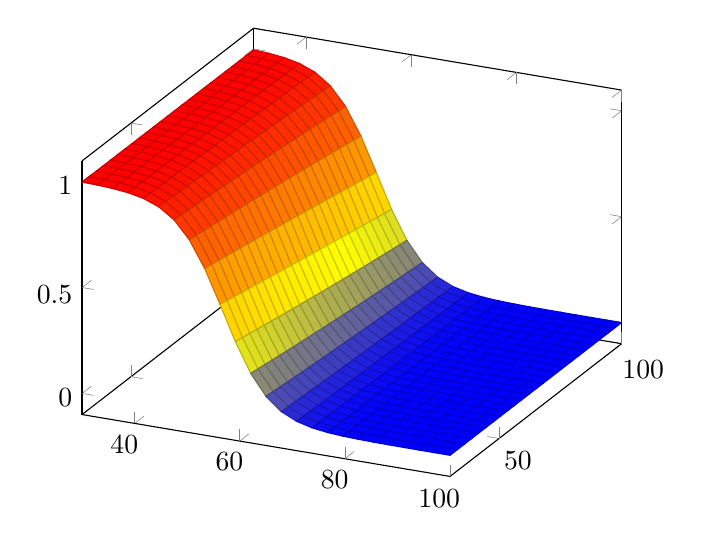
\begin{tikzpicture}
    \begin{axis}
    \addplot3[
        surf,
        domain=30:100
    ]
    {exp(13.29236 -0.22867*x-0.01040*y)/(1+exp(13.29236 -0.22867*x-0.01040*y))};
    \end{axis}
\end{tikzpicture}
\caption{Izračunane verjetnosti z dvema pojasnjevalnima spremenljivkama}
\end{figure}
\end{center}
Zopet smo algoritem pognali na enakih začetnih vrednostih približka in zahtevane natančnosti, rešitev pa dobili po štirih iteracijah.

\subsection{Ocenjevanje parametrov v probit modelu}
Sedaj ponovimo postopek še s probit modelom. Zaradi neoptimizirane numerične metode pričakujemo večje število iteracij za doseženo želeno natančnost.

\subsubsection{Algoritem za probit model}
Najprej postavimo algoritem. Ta se idejno sicer ne bo bistveno razlikoval od tistega uporabljenega v prejšnjem odseku, vendar pa je očitno precej bolj zapleten za računanje.
Posebej smo označili \textit{koeficiente} pri Hessejevi matriki in funkciji zbira - to so le deli dejanske formule, izračunani posebej za večjo preglednost.

\begin{algorithm}[H]
    \caption{\textbf{function} ProbitModel(iteracije, X, Y, $\beta_{zacetni}$, $\epsilon$)}
\begin{algorithmic}

    \STATE $p = \Phi(X^\top \beta_{zacetni})$
    \STATE $Score_{koef} = \frac{Y-p}{p*(1-p)} * \phi(X^\top \beta_{zacetni})$
    \STATE $Score = X^\top Score_{koef}$

    %\STATE $Hess_{koef} = \frac{\phi(X^\top \beta_{zacetni})}{p*(1-p)} * \left(\phi(X^\top \beta_{zacetni})\frac{2*p*Y - p^2-Y}{p*(1-p)} - X(Y - p)\right)$
    \STATE $Hess_{koef} =\frac{(Y-p)(-\phi(X^\top \beta_{zacetni})X^\top \beta_{zacetni} - \phi(X^\top \beta_{zacetni}))}{p(1-p)} - \frac{\phi(X^\top \beta_{zacetni})^2(1-2p)}{(p(1-p))^2}$
    \STATE $Hess = diag(Hess_{koef})$
    \STATE $H = X^\top Hess_{koef} X$
        
    \STATE \text{\textit{Reši sistem na h:}} $H * h = Score$
    \STATE $\beta_{star} = \beta_{zacetni}$
    \STATE $\beta_{nov} = \beta_{star} - h$
    \WHILE{$i \leq \text{iteracije}$}
        
        \IF{$\beta_{nov} - \beta_{star} \geq \epsilon$}
            \STATE $p = \Phi(X^\top \beta_{nov})$
            \STATE $Score_{koef} = \frac{Y-p}{p*(1-p)} * \phi(X^\top \beta_{nov})$
            \STATE $Score = X^\top Score_{koef}$
            
            \STATE $Hess_{koef} = \frac{\phi(X^\top \beta_{nov})}{p*(1-p)} * \left(\phi(X^\top \beta_{nov})\frac{2*p*Y - p^2-Y}{p*(1-p)} - X(Y - p)\right)$
            \STATE $H = X^\top Hess_{koef} X$
            \STATE \text{\textit{Razreši na h:}}
            \STATE $H * h = Score$ 
            \STATE $\beta_{star} = \beta_{nov}$ 
            \STATE $\beta_{nov} = \beta_{star} - h$ 
        \ELSE
        \STATE \text{\textit{Dosegli smo želeno natančnost v zadostnem številu korakov}}
        \RETURN $\beta_{nov}$
        \ENDIF
        
    \ENDWHILE
\end{algorithmic}
\end{algorithm}
Ponovimo postopek in za oceno le z eno pojasnjevalno spremenljivko po vsega petih iteracijah dobimo $\beta_{0} = 8.77495,~\beta_{1} = -0.13510$ in funkcijo
\[
    \frac{e^{8.77495-0.13510x}}{1+e^{8.77495-0.13510x}}.
\]
Za vključeni obe spremenljivki pa $\beta_{0} = 8.08004,~\beta_{1} = -0.13774,~\beta_{2} = -0.006014$

Torej je predvidevanje, da bomo potrebovali bistveno več iteracij, napačno, saj je bila potrebna le ena več kot pri logistični regresiji. Ugibamo, da do tega pride zaradi
majhne količine testnih podatkov in bi se pri večjih podatkovnih bazah razlike primerno povečale.

\subsection{Primerjava logit in probit modela}
Oglejmo si še direktno primerjavo dobljenih rezultatov.
\begin{center}
    \begin{figure}[H]
    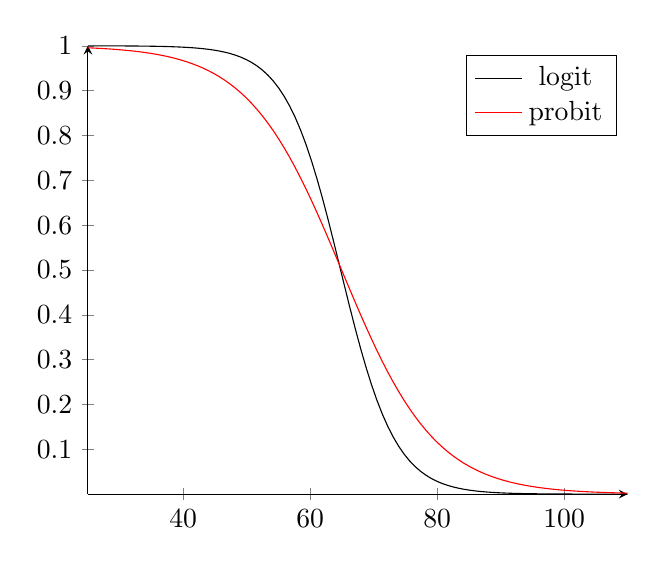
\begin{tikzpicture}
        \begin{axis}[
            axis lines = center,
            %xtick = {-10,-9,-8,...,9,10}
            ytick = {0,0.1,0.2,...,1,1.1,1.2,1.3,1.4},
            %ylabel = verjetnost,
            %y label style = {at={(axis description cs:0.25,.5)},rotate=90}%,anchor=south}
        ]
        \addplot [
            domain=25:110, 
            samples=100, 
            color=black,
            ]
            {exp(15.04290 - (0.23216 * x))/(1 + exp(15.04290 - (0.23216 * x)))};
        \addplot[
            domain=25:110, 
            samples=100,
            color = red,
            ]
            {exp(8.77495 - (0.13510 * x))/(1 + exp(8.77495 - (0.13510 * x)))};
        %\addlegendentry{$x^2 + 2x + 1$}
        \addlegendentry{logit}
        \addlegendentry{probit}
        \end{axis}
    \end{tikzpicture}
    \caption{Izračunane verjetnosti z eno pojasnjevalno spremenljivko}
    \label{fig:logit2}
    \end{figure}
    \end{center}

Z rdečo je na zgornjem grafu narisana sigmoida, dobljena iz probit modela, s črno pa iz logističnega. Kljub temu da se število iteracij za njun izračun ne razlikuje
bistvemo, bi v tem primeru raje izbrali logistični model. Razlog tiči v hitrosti padanja, ki je višja pri slednjem, kar nam koristi pri nadaljnji analizi.
% slovar
\section*{Slovar strokovnih izrazov}
\geslo{generalized linear model}{posplošeni linearni model}

\geslo{score function}{funkcija zbira}

\geslo{Fisher's scoring}{Fisherjeva zbirna metoda}

\geslo{Fisher information matrix}{Fisherjeva informacijska matrika}

\geslo{link function}{povezovalna funkcija}

\geslo{maximum likelihood estimator (MLE)}{cenilka največjega verjetja}

\geslo{exponential family}{eksponentna družina}
%
%
% seznam uporabljene literature
%\begin{thebibliography}{99}
%\bibitem{}
%end{thebibliography}
\nocite{*}
\bibliographystyle{plain}
\bibliography{literatura}



\end{document}
